%!TEX TS-program = xelatex
\documentclass[notes,12pt, aspectratio=169]{beamer}

\usepackage{amsmath,amsfonts,amssymb,amsthm,mathtools}  % пакеты для математики
%\usepackage{minted}

\usepackage[english, russian]{babel} % выбор языка для документа
\usepackage[utf8]{inputenc} % задание utf8 кодировки исходного tex файла
\usepackage[X2,T2A]{fontenc}        % кодировка

\usepackage{fontspec}         % пакет для подгрузки шрифтов
\setmainfont{Helvetica}  % задаёт основной шрифт документа

% why do we need \newfontfamily:
% http://tex.stackexchange.com/questions/91507/
\newfontfamily{\cyrillicfonttt}{Helvetica}
\newfontfamily{\cyrillicfont}{Helvetica}
\newfontfamily{\cyrillicfontsf}{Helvetica}

\usepackage{unicode-math}     % пакет для установки математического шрифта
% \setmathfont{Neo Euler} % шрифт для математики

\usepackage{polyglossia}      % Пакет, который позволяет подгружать русские буквы
\setdefaultlanguage{russian}  % Основной язык документа
\setotherlanguage{english}    % Второстепенный язык документа

% Шрифт для кода
\setmonofont[Scale=0.85]{Monaco}
\usepackage{verbments}

\usepackage{pgfpages}
% These slides also contain speaker notes. You can print just the slides,
% just the notes, or both, depending on the setting below. Comment out the want
% you want.
%\setbeameroption{hide notes} % Only slide
%\setbeameroption{show only notes} % Only notes
%\setbeameroption{show notes on second screen=right} % Both

\usepackage{array}

\usepackage{tikz}
\usepackage{verbatim}
\setbeamertemplate{note page}{\pagecolor{yellow!5}\insertnote}
\usetikzlibrary{positioning}
\usetikzlibrary{snakes}
\usetikzlibrary{calc}
\usetikzlibrary{arrows}
\usetikzlibrary{decorations.markings}
\usetikzlibrary{shapes.misc}
\usetikzlibrary{matrix,shapes,arrows,fit,tikzmark}

\usepackage{hyperref}
\usepackage{lipsum}
\usepackage{multimedia}
\usepackage{multirow}
\usepackage{dcolumn}
\usepackage{bbm}
\newcolumntype{d}[0]{D{.}{.}{5}}

\usepackage{changepage}
\usepackage{appendixnumberbeamer}
\newcommand{\beginbackup}{
   \newcounter{framenumbervorappendix}
   \setcounter{framenumbervorappendix}{\value{framenumber}}
   \setbeamertemplate{footline}
   {
     \leavevmode%
     \hline
     box{%
       \begin{beamercolorbox}[wd=\paperwidth,ht=2.25ex,dp=1ex,right]{footlinecolor}%
%         \insertframenumber  \hspace*{2ex} 
       \end{beamercolorbox}}%
     \vskip0pt%
   }
 }
\newcommand{\backupend}{
   \addtocounter{framenumbervorappendix}{-\value{framenumber}}
   \addtocounter{framenumber}{\value{framenumbervorappendix}} 
}

% для имитации питоновского синтаксиса 
\newcommand{\pgr}[1]{{\color{green} \textbf{#1}}}


%%%%%%%%%% Работа с картинками %%%%%%%%%
\usepackage{graphicx}                  % Для вставки рисунков
\usepackage{graphics}
\graphicspath{{images/}}    % можно указать папки с картинками
\usepackage{wrapfig}                   % Обтекание рисунков и таблиц текстом

\usepackage[space]{grffile}
\usepackage{booktabs}

% These are my colors -- there are many like them, but these ones are mine.
\definecolor{blue}{RGB}{0,114,178}
\definecolor{red}{RGB}{213,94,0}
\definecolor{yellow}{RGB}{240,228,66}
\definecolor{green}{RGB}{0,128, 0}

\hypersetup{
  colorlinks=false,
  linkbordercolor = {white},
  linkcolor = {blue}
}


%% I use a beige off white for my background
\definecolor{MyBackground}{RGB}{255,253,218}

%% Uncomment this if you want to change the background color to something else
%\setbeamercolor{background canvas}{bg=MyBackground}

%% Change the bg color to adjust your transition slide background color!
\newenvironment{transitionframe}{
  \setbeamercolor{background canvas}{bg=yellow}
  \begin{frame}}{
    \end{frame}
}

\setbeamercolor{frametitle}{fg=blue}
\setbeamercolor{title}{fg=black}
\setbeamertemplate{footline}[frame number]
\setbeamertemplate{navigation symbols}{} 
\setbeamertemplate{itemize items}{-}
\setbeamercolor{itemize item}{fg=blue}
\setbeamercolor{itemize subitem}{fg=blue}
\setbeamercolor{enumerate item}{fg=blue}
\setbeamercolor{enumerate subitem}{fg=blue}
\setbeamercolor{button}{bg=MyBackground,fg=blue,}


% If you like road maps, rather than having clutter at the top, have a roadmap show up at the end of each section 
% (and after your introduction)
% Uncomment this is if you want the roadmap!
% \AtBeginSection[]
% {
%    \begin{frame}
%        \frametitle{Roadmap of Talk}
%        \tableofcontents[currentsection]
%    \end{frame}
% }
\setbeamercolor{section in toc}{fg=blue}
\setbeamercolor{subsection in toc}{fg=red}
\setbeamersize{text margin left=1em,text margin right=1em} 

% списки, которые растягиваются на всю величину слайда 
\newenvironment{wideitemize}{\itemize\addtolength{\itemsep}{10pt}}{\enditemize}

\DeclareMathOperator{\Var}{Var}
\DeclareMathOperator{\E}{E}

\title[]{\textcolor{blue}{Глубокое обучение и вообще}}
\author{Ульянкин Филипп}
\date{\today}

\usepackage[normalem]{ulem}

\begin{document}

%%% TIKZ STUFF
\tikzset{   
        every picture/.style={remember picture,baseline},
        every node/.style={anchor=base,align=center,outer sep=1.5pt},
        every path/.style={thick},
        }
\newcommand\marktopleft[1]{%
    \tikz[overlay,remember picture] 
        \node (marker-#1-a) at (-.3em,.3em) {};%
}
\newcommand\markbottomright[2]{%
    \tikz[overlay,remember picture] 
        \node (marker-#1-b) at (0em,0em) {};%
}
\tikzstyle{every picture}+=[remember picture] 
\tikzstyle{mybox} =[draw=black, very thick, rectangle, inner sep=10pt, inner ysep=20pt]
\tikzstyle{fancytitle} =[draw=black,fill=red, text=white]
%%%% END TIKZ STUFF

% Title Slide


\begin{frame}
\maketitle
\centering \textbf{\color{blue} Посиделка 5:}  Нейросети — конструктор LEGO
\end{frame}


\begin{frame}{Agenda}
\begin{wideitemize}
	\item  Какими бывают функции активации
	\item  Паралич  нейронной сети и взрыв градиентов 
	\item  Инициализация весов 
	\item  Переобучение нейронных сетей
	\item  Регуляризация: $l_1, l_2$, дропаут, ранняя остановка, их взаимосвязь
	\item  Первая порция советов по обучению нейросетей 	
\end{wideitemize} 
\end{frame}


\begin{transitionframe}
	\begin{center}
		\Huge Какими бывают функции активации
	\end{center}
	\centering 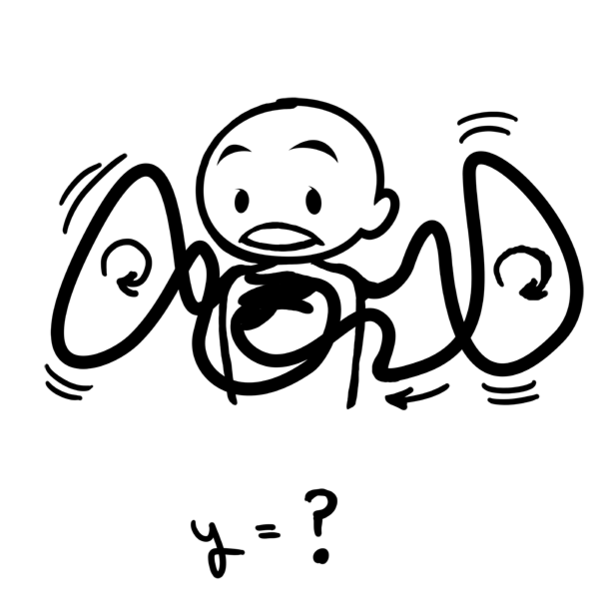
\includegraphics[scale = 0.15]{act_f.png}
\end{transitionframe}


\begin{frame}{Сигмоида (sigmoid activation)}
\begin{center}
	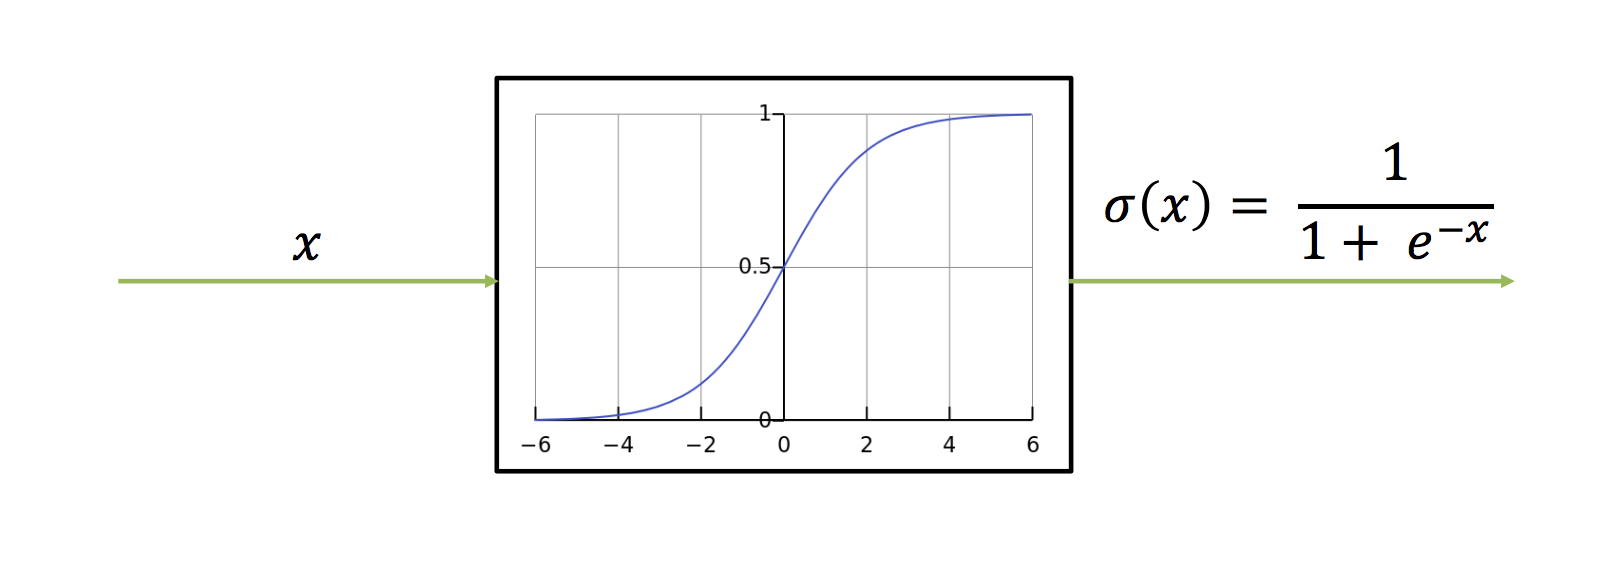
\includegraphics[width=.9\linewidth]{sigmoid_activation_1.png}
\end{center}
\end{frame}


\begin{frame}{Сигмоида (sigmoid activation)}
\begin{center}
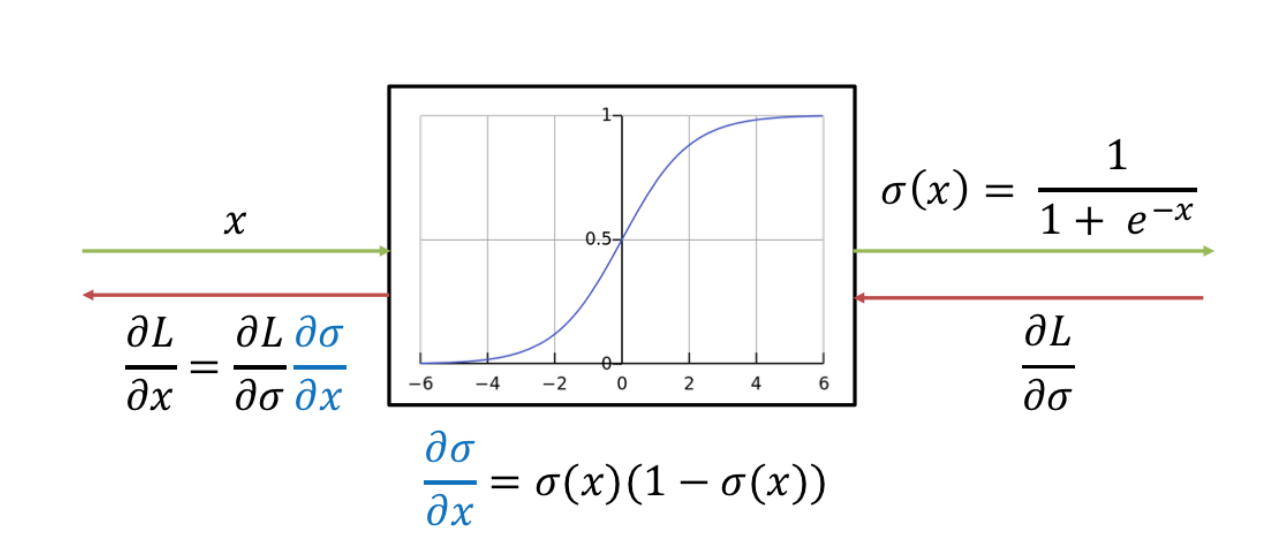
\includegraphics[width=.8\linewidth]{sigmoid_activation_2.png}
\end{center}
\end{frame}


\begin{frame}{Сигмоида (sigmoid activation)}
\begin{center}
	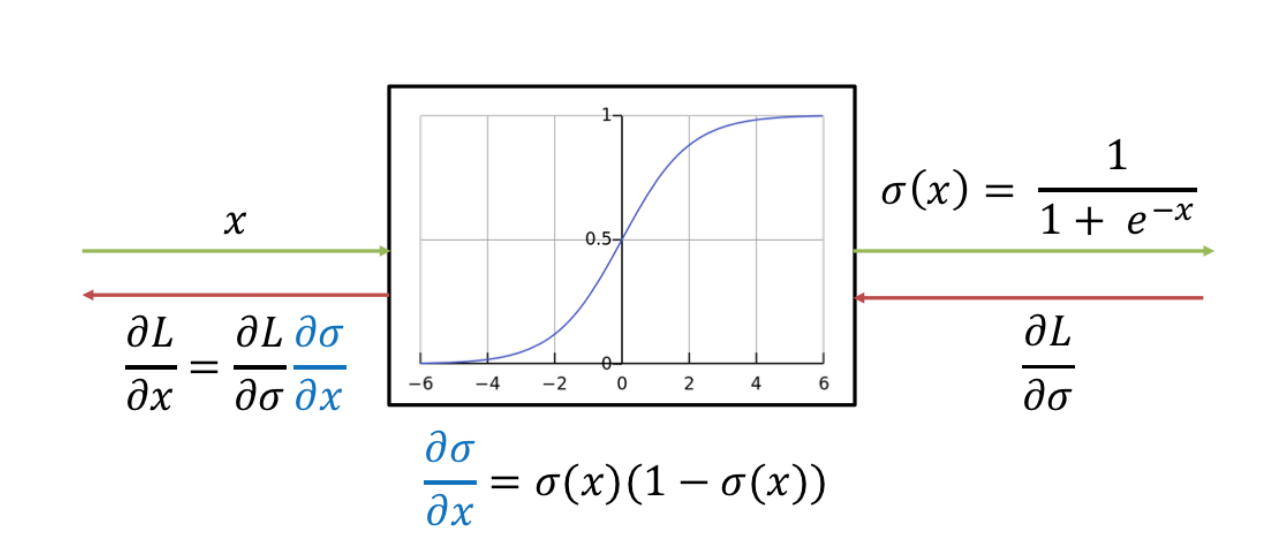
\includegraphics[width=.65\linewidth]{sigmoid_activation_2.png}
\end{center}

\begin{itemize}
	\item Сигмоида была популярна как классическая функция активации, но у неё есть ряд проблем
	{\color{red} 
	\item Насыщенные нейроны зануляют градиенты, в глубоких сетях возможен паралич
	}
\end{itemize}
\end{frame}


\begin{frame}{Затухание градиента (vanishing gradient problem)}
\begin{columns}
	\begin{column}{0.45\textwidth}
		\begin{wideitemize}
			\item  Изменение параметров в ходе обучения происходит на величину, которая  не влияет на выход сети
			
			\item Проблема связана с очень маленькими градиентами при обновлении весов:
			
			$$
			w_t = w_{t-1} - \gamma \cdot \nabla L(w_{t-1})
			$$
			
			\item При насыщении сети сигмоида убивает градиенты
		\end{wideitemize}
	\end{column}
	\hfill
	\begin{column}{0.55\textwidth}
		
		\begin{center}
			\only<1>{ 
				$$
				f(t) = \frac{1}{1 + e^{-t}}
				$$
				
				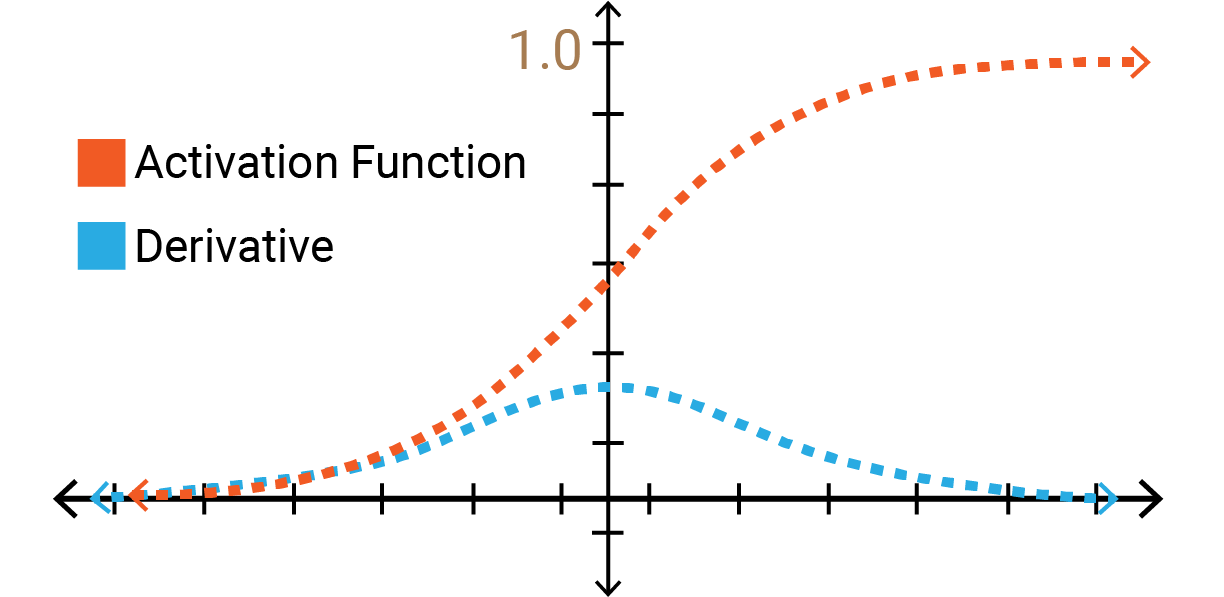
\includegraphics[width=0.98\textwidth]{sigm_der.png} 
			}
			
			% Сделать тут нормальную картинку 
			\only<2>{
				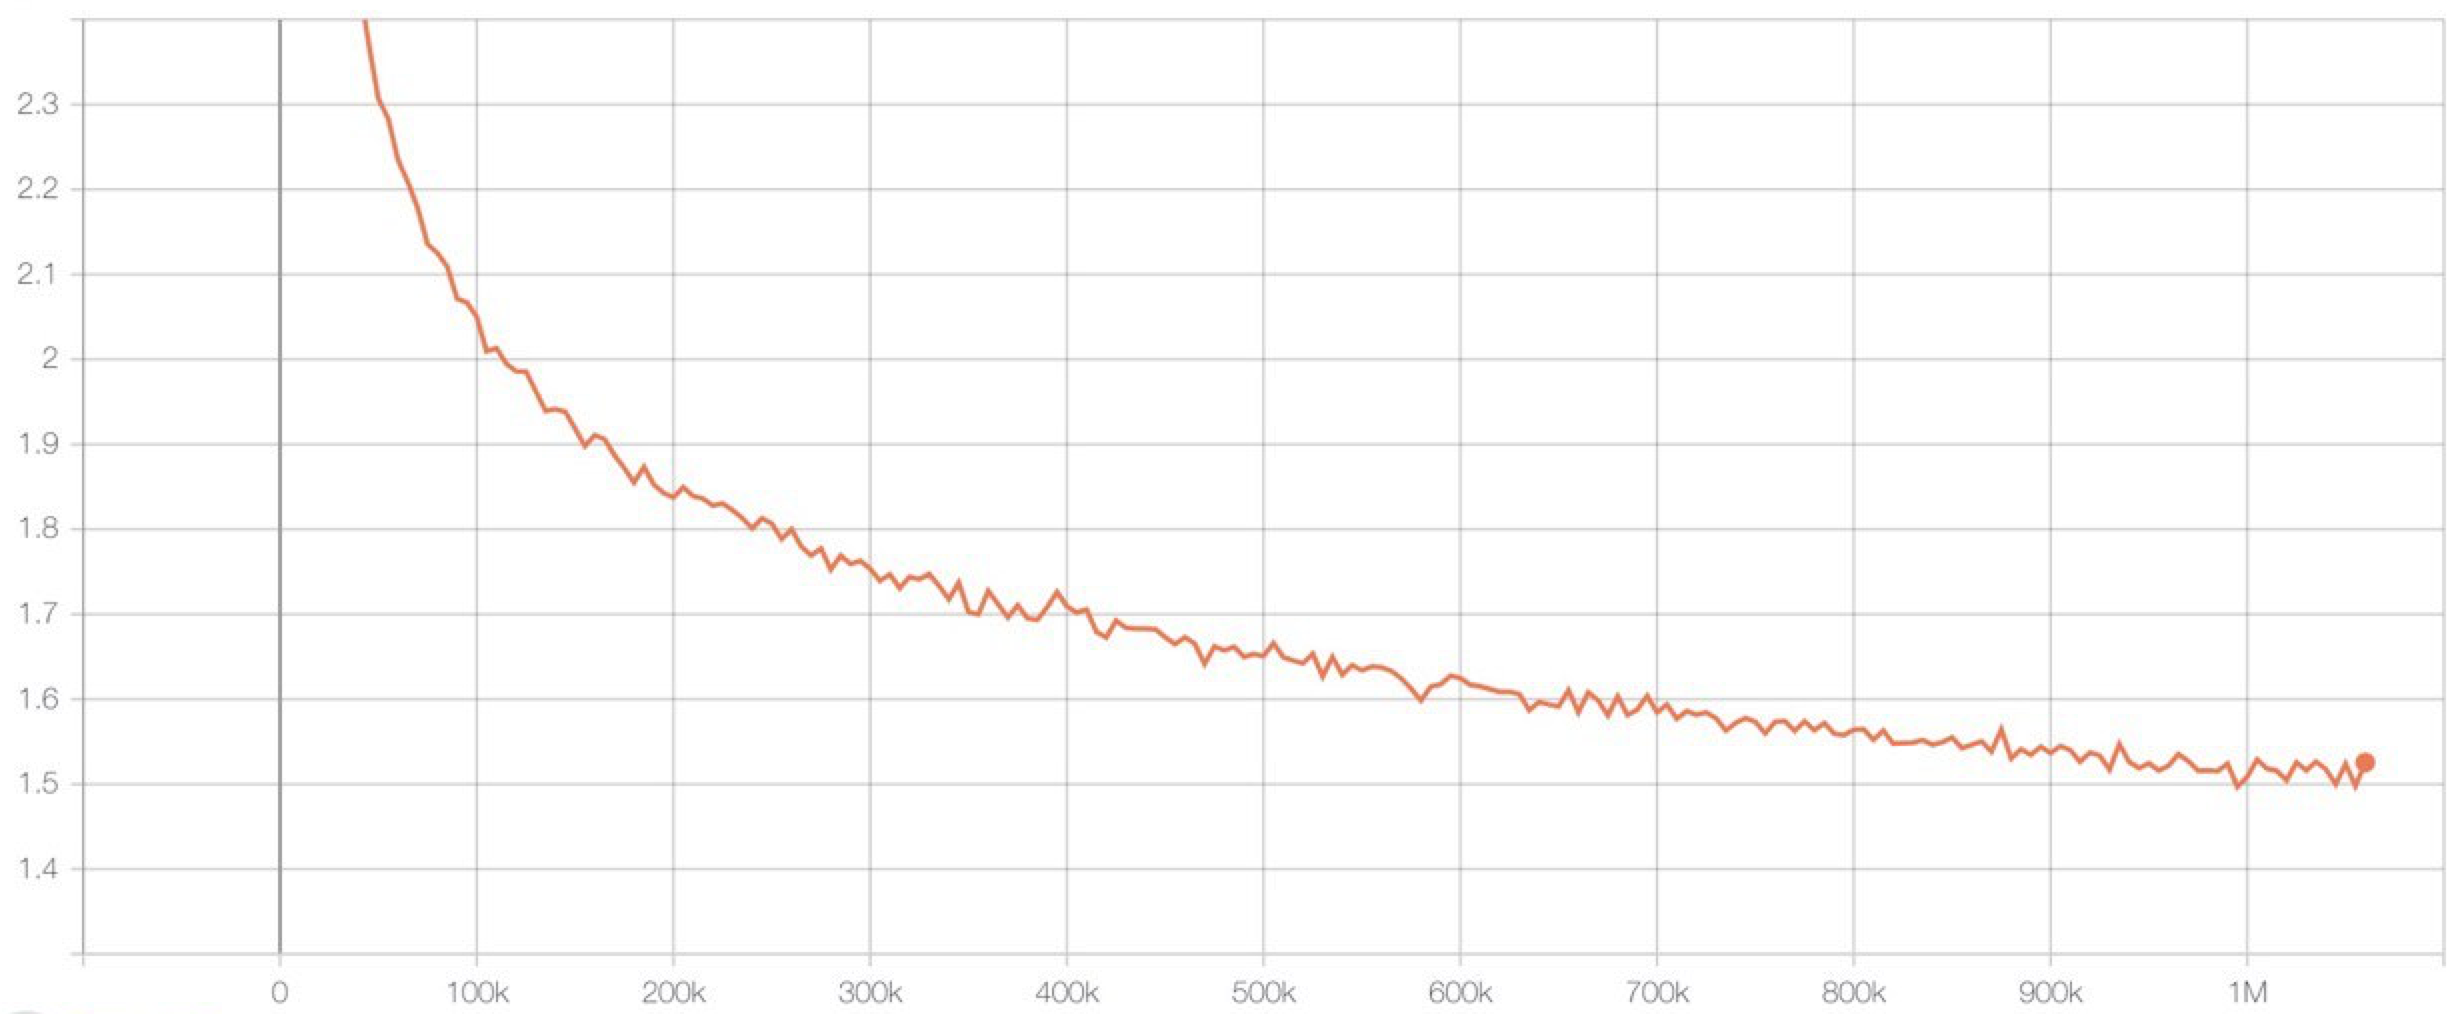
\includegraphics[width=0.98\textwidth]{vanishing_loss.png} 
				
				\mbox{  }
				
				\alert{Толи обучение сошлось, толи веса просто больше не обновляются \ldots}
			}
		\end{center} 
	\end{column}
\end{columns}
\end{frame}


\begin{frame}{Паралич сети}
	\begin{wideitemize}
		\item  В случае сигмоиды $\sigma'(x) = \sigma(x) \cdot (1 - \sigma(x))$ 
		
		\item Сигмоида принимает значения на отрезке $[0; 1]$, значит максимальное значение её производной это $^1/_4$
		
		\item Если сеть очень глубокая, происходит \alert{затухание градиента} 
		
		\item Градиент затухает экспоненциально $\Rightarrow$ сходимость замедляется, более ранние веса обновляются дольше, более глубокие веса быстрее  $\Rightarrow$ значение градиента становится ещё меньше $\Rightarrow$ наступает \alert{паралич сети} 
		
		\item В сетях с небольшим числом слоёв этот эффект незаметен
	\end{wideitemize} 
\end{frame}


\begin{frame}{Взрыв градиента (exploding gradient problem)}
\begin{columns}
	\begin{column}{0.4\textwidth}
		\begin{wideitemize}
			\item  Изменение параметров в ходе обучения происходит на очень большую величину и обучение деградирует
			
			\item Проблема связана с очень большими градиентами при обновлении весов:
			
			$$
			w_t = w_{t-1} - \gamma \cdot \nabla L(w_{t-1})
			$$
			
		\end{wideitemize}
	\end{column}
	\hfill
	\begin{column}{0.6\textwidth}
		
		\begin{center}
				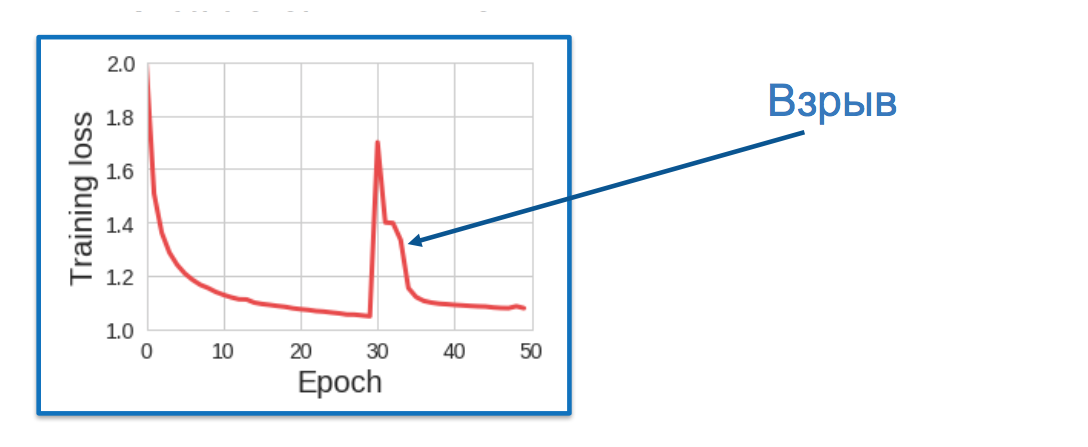
\includegraphics[width=0.98\textwidth]{exp_grad.png} 
		\end{center} 
	\end{column}
\end{columns}
\end{frame}


\begin{frame}{Взрыв и затухание градиента}
	\begin{wideitemize}
		\item Затухание градиента связано не только с сигмоидой
		\item Взрыв градиента также встречается довольно часто 
		\item $\Rightarrow$ грамотные инициализация и оптимизация
		\item $\Rightarrow$ разработка новых архитектур и специальных слоёв
	\end{wideitemize}
\end{frame}


\begin{frame}{Сигмоида (sigmoid activation)}
\begin{center}
	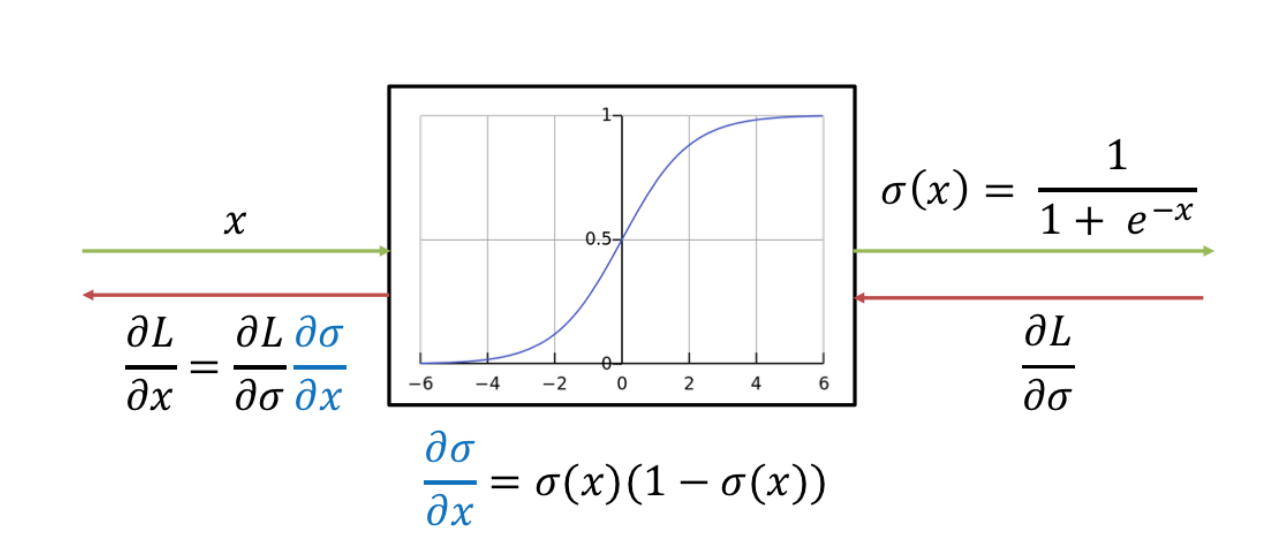
\includegraphics[width=.65\linewidth]{sigmoid_activation_2.png}
\end{center}

\begin{itemize}
	{\color{red} 
		\item Насыщенные нейроны зануляют градиенты, в глубоких сетях возможен паралич
		\item Не центрирована относительно нуля
	}
		\item Что мы можем сказать о градиентах нейрона с сигмоидой? 
\end{itemize}
\end{frame}


\begin{frame}{Центрирование относительно нуля}
\begin{columns}
	\begin{column}{0.6\textwidth}
		\begin{wideitemize}
			\item  Выход слоя мы обычно находим как 
			
			\[
			o_i = \sigma(h_i)
			\]
			
			\item он всегда положительный, значит градиент по весам, идущим на вход в текущий нейрон тоже положительные 
			\item $\Rightarrow$ все веса обновляются в одинаковом направлении 
			\item $\Rightarrow$ сходимость идёт медленнее, причём зиг-загами
		\end{wideitemize} 
	\end{column}
	\hfill
	\begin{column}{0.4\textwidth}
		
		\begin{center}
			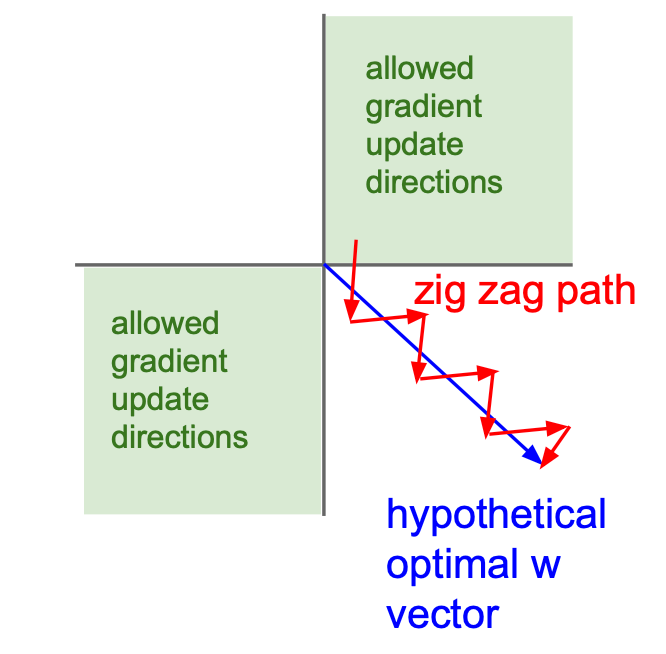
\includegraphics[width=0.98\textwidth]{gr_update.png} 
		\end{center} 
	\end{column}
\end{columns}
\end{frame}



\begin{frame}{Сигмоида (sigmoid activation)}
\begin{center}
	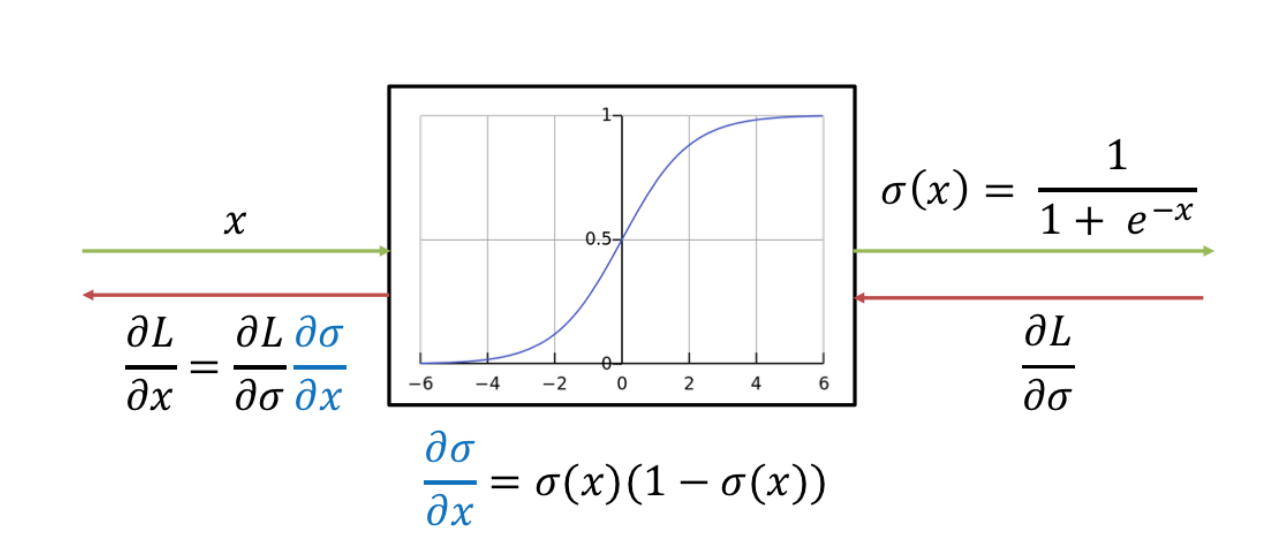
\includegraphics[width=.65\linewidth]{sigmoid_activation_2.png}
\end{center}

\begin{itemize}
	{\color{red} 
		\item Насыщенные нейроны зануляют градиенты, в глубоких сетях возможен паралич
		\item Не центрирована относительно нуля
		\item Вычислять $e^x$ дорого
	}
\end{itemize}
\end{frame}


\begin{frame}{Гиперболический тангенс (tanh activation)}
	\begin{center}
		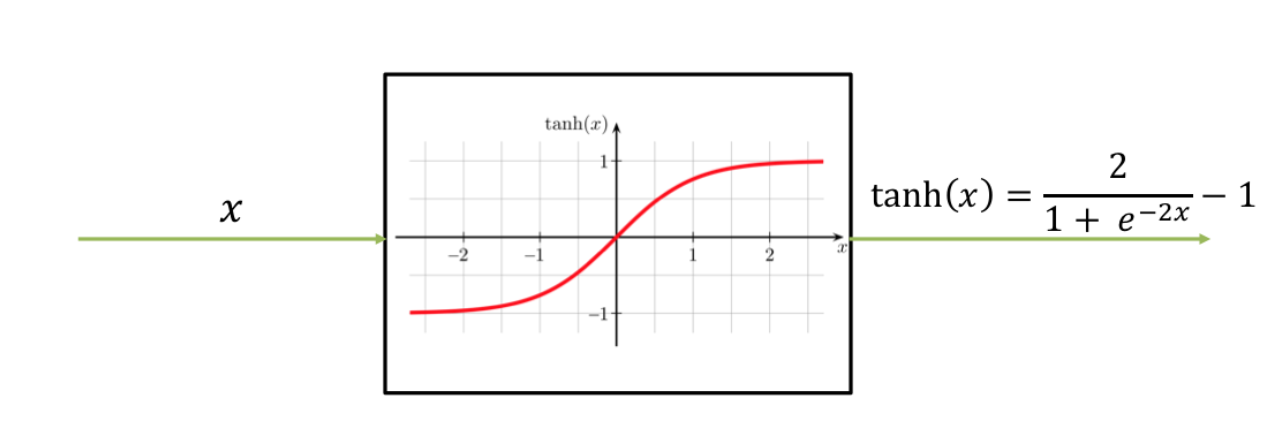
\includegraphics[width=.8\linewidth]{tanh_activation.png}
	\end{center}
	\begin{itemize}
		\item  {\color{green}  Центрирован относительно нуля }
		
		\item  {\color{red}  Всё ещё похож на сигмоиду }
		
		\item $f'(x) = 1 - f(x)^2$  $\Rightarrow$ затухание градиента
	\end{itemize}
\end{frame}


\begin{frame}{Rectifier Linear Unit activation, ReLU (2012)}
	\begin{center}
		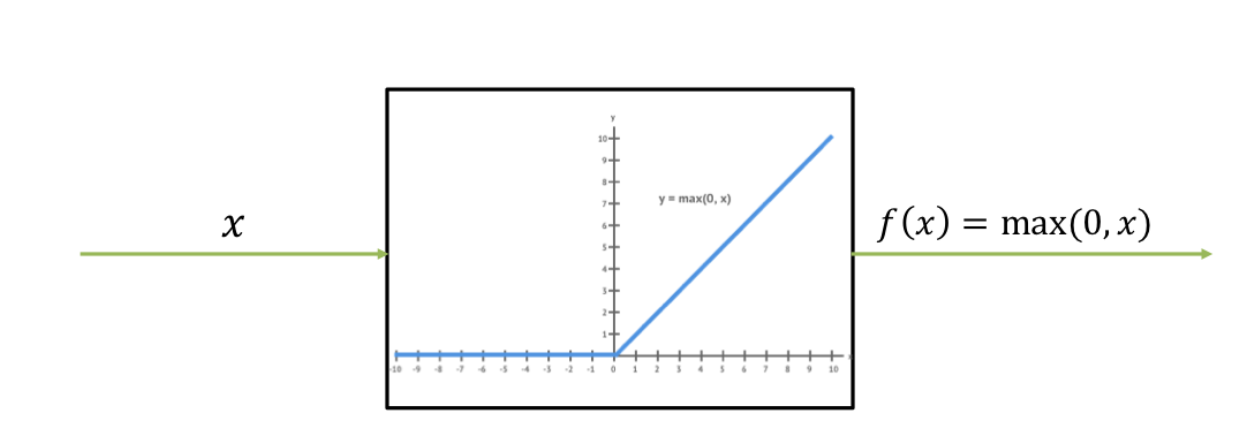
\includegraphics[width=.8\linewidth]{relu_activation.png}
	\end{center}
	\begin{itemize}
		{ \color{green} 
		\item  Быстро вычисляется 
		\item  Градиенты не угасают при $x > 0$
		\item  На практике ускоряет сходимость
		} 
	\end{itemize}
\end{frame}


\begin{frame}{ReLU (2012)}
	\begin{center}
		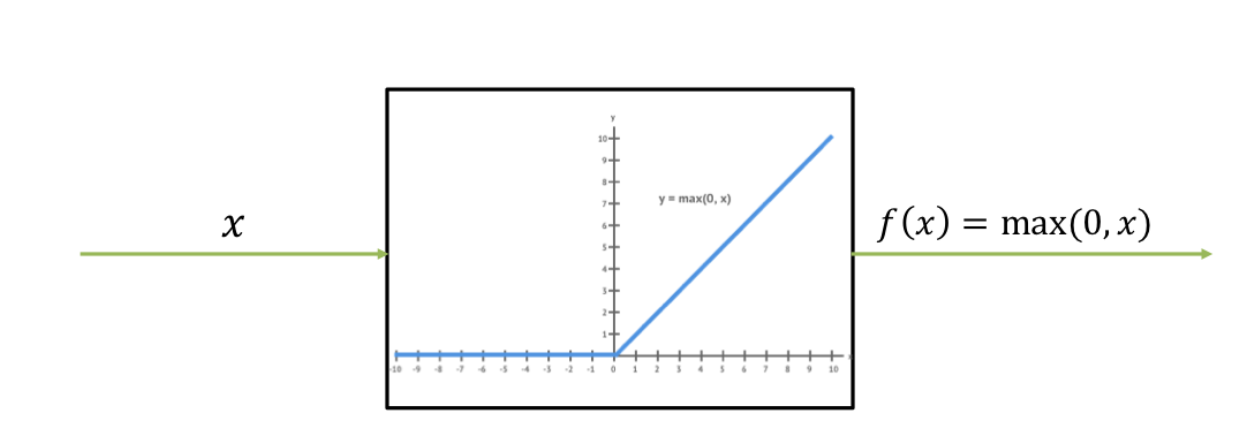
\includegraphics[width=.8\linewidth]{relu_activation.png}
	\end{center}
	\begin{itemize}
		{ \color{red} 
		\item  Сетка может умереть, если активация занулится на всех нейронах
		\item  Не центрирован относительно нуля
		} 
	\end{itemize}
\end{frame}


\begin{frame}{Зануление ReLU}
	\begin{center}
		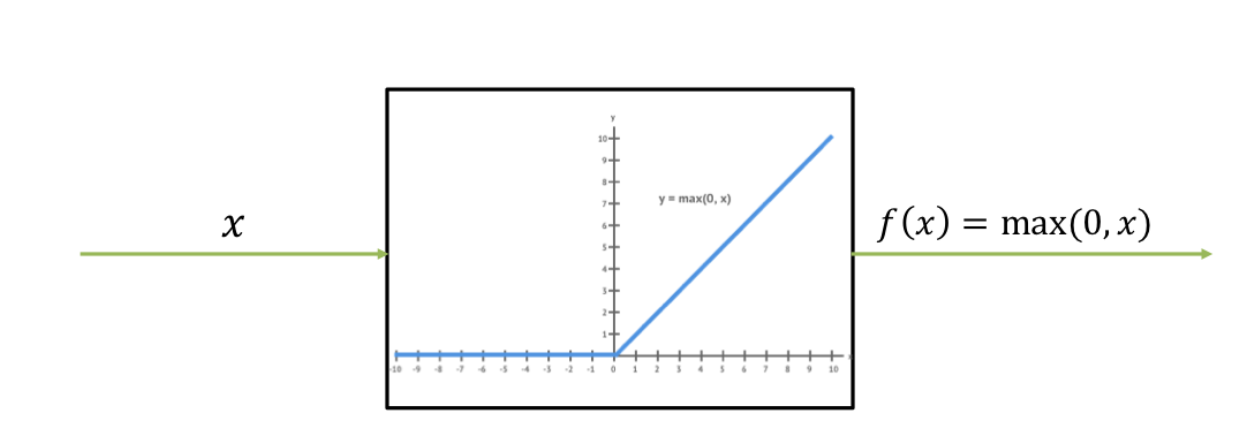
\includegraphics[width=.8\linewidth]{relu_activation.png}
	\end{center}
	\begin{wideitemize}
		\item   $f(x) = \max(0, w_0 + w_1 \cdot h_1 + \ldots + w_k \cdot h_k)$
		
		\item  Если $w_0$ инициализировано большим отрицательным числом, нейрон сразу умирает $\Rightarrow$ надо аккуратно инициализировать веса
	\end{wideitemize}
\end{frame}


\begin{frame}{Leaky ReLU activation (2013)}
\begin{center}
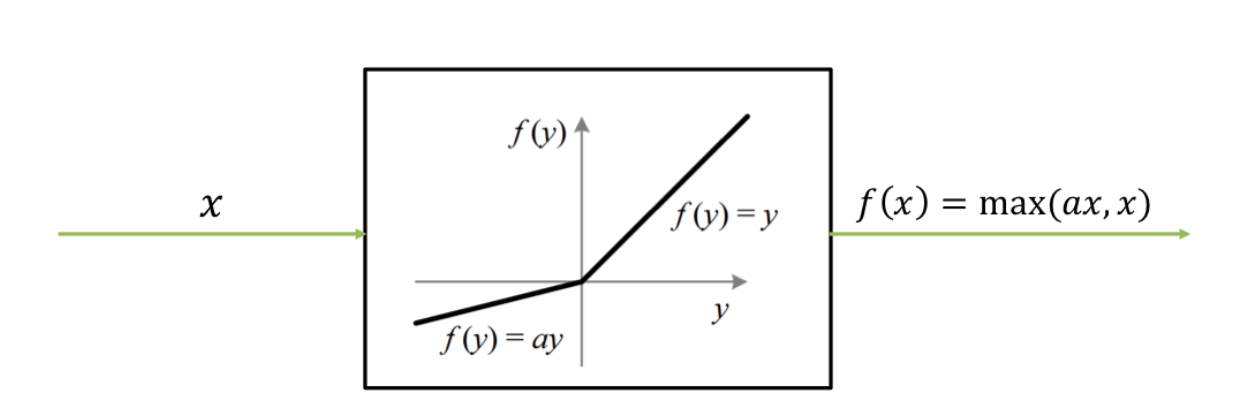
\includegraphics[width=.8\linewidth]{leaky_relu_activation.png}
\end{center}

\begin{itemize}
{ \color{green} 
\item Как ReLU, но не умирает, всё ещё легко считается
\item Производная может быть любого знака
\item Важно, чтобы $a \ne 1$, иначе линейность} 
{\color{red} 
\item  Не центрирован относительно нуля} 
\end{itemize}
\end{frame}


\begin{frame}{Exponential Linear Units activation, ELU (2015)}
	\begin{center}
		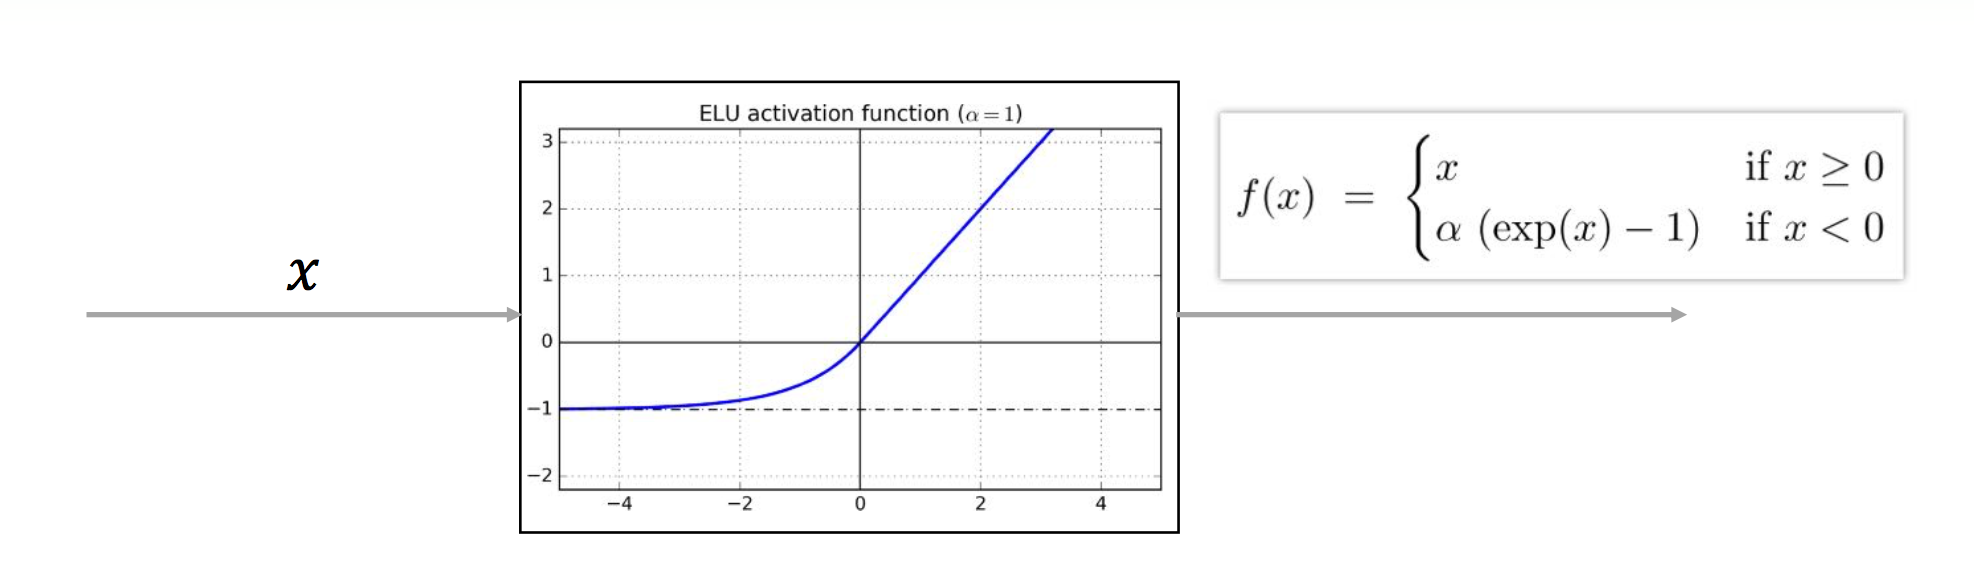
\includegraphics[width=.8\linewidth]{elu.png}
	\end{center}
	\begin{columns}
		\begin{column}{0.7\textwidth}
			\begin{itemize}
				{ \color{green} 
					\item  Примерно центрирован в нуле (в контексте математического ожидания)
					\item  Сходимость быстрее ReLU
					\item  На практике ускоряет сходимость} 
			\end{itemize}
		\end{column}
		\hfill
		\begin{column}{0.4\textwidth}
			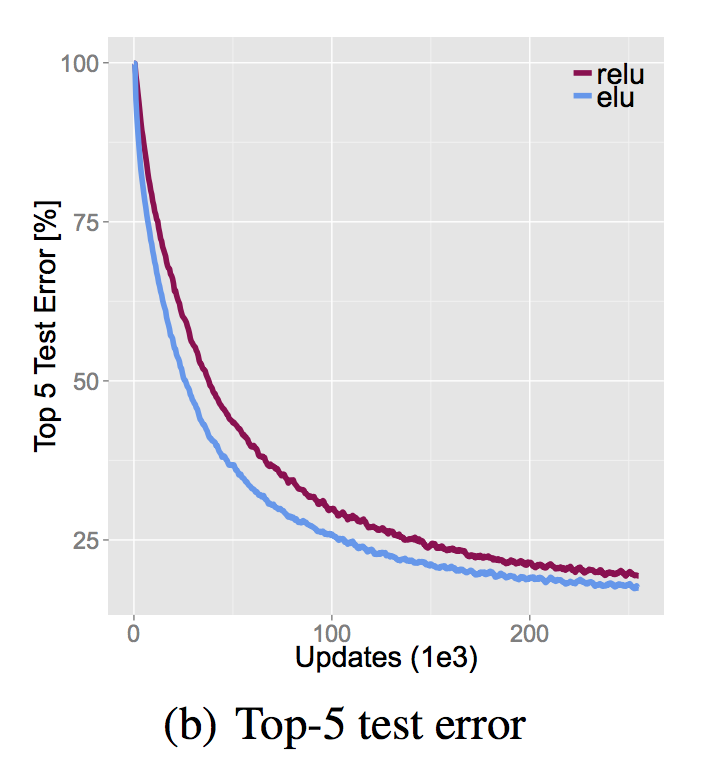
\includegraphics[width=.55\linewidth]{elu_loss.png}
		\end{column}
	\end{columns}
\vfill %
\footnotesize
{\color{blue} \url{https://arxiv.org/pdf/1511.07289.pdf}}
\end{frame}


\begin{frame}{Scaled Exponential Linear Units activation, SELU (2017)}
\begin{columns}
	\begin{column}{0.45\textwidth}
		\begin{center}
			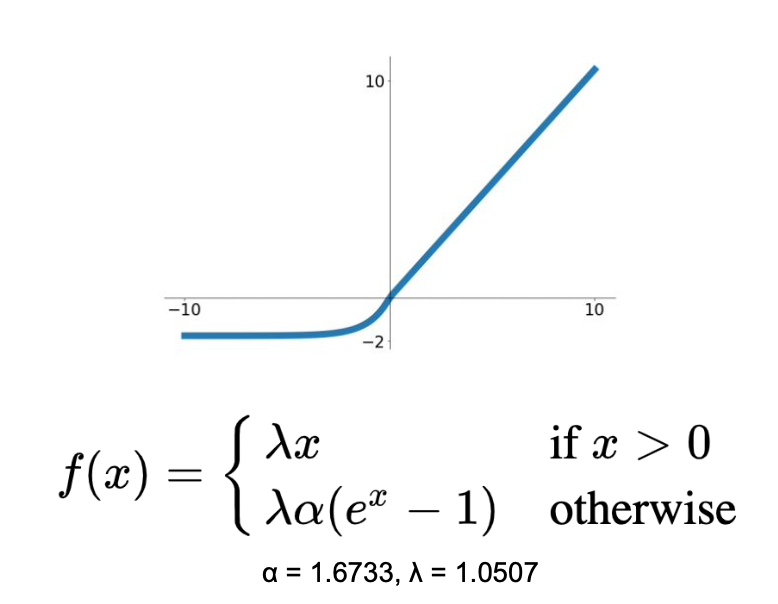
\includegraphics[width=.99\linewidth]{selu.png}
		\end{center}
	\end{column}
	\hfill
	\begin{column}{0.55\textwidth}
		\begin{wideitemize} 
				\item  Нормализованная версия ELU, лучше работает для глубоких сетей
				\item  Обладает свойством самонормализации
				\item  Можно учить сетки без нормализации по батчам (будем обсуждать позже)
		\end{wideitemize}
	\end{column}
\end{columns}
\vfill %
\footnotesize
{\color{blue} \url{https://arxiv.org/abs/1706.02515}}
\end{frame}

\begin{frame}{Swish (2017)}
	\begin{columns}
		\begin{column}{0.35\textwidth}
			\begin{center}
				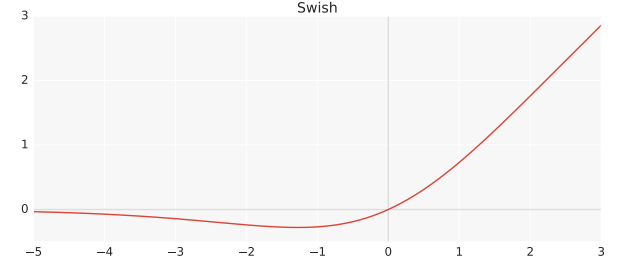
\includegraphics[width=.95\linewidth]{swish.png}
				\[f(x) = x \cdot \sigma(\beta x) \]
			\end{center}
		\mbox{    } параметр $\beta$ обучается
		\end{column}
		\hfill
		\begin{column}{0.65\textwidth}
			\begin{itemize} 
				\item  В 2017 году Google Brain хитрым автоматическим поиском на основе RNN нашла функцию активации Swish, работающую лучше ReLU
			\end{itemize}
		\begin{center}
			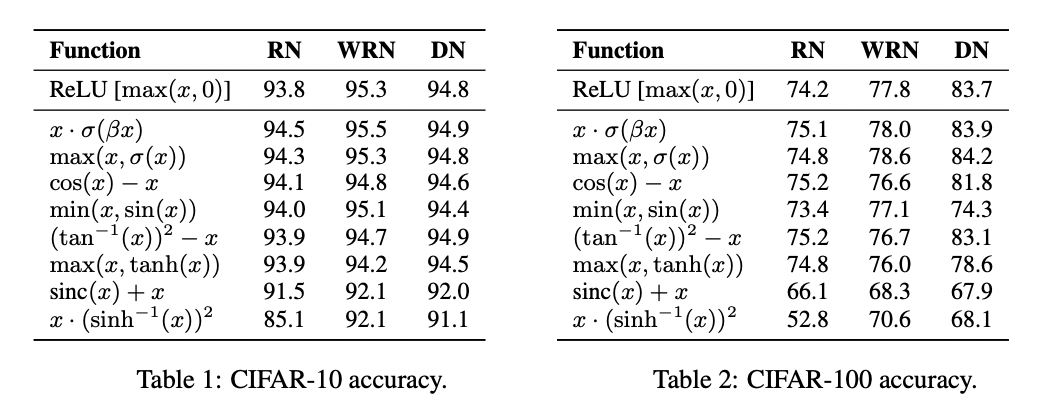
\includegraphics[width=.99\linewidth]{swish_can.png}
		\end{center}
		\end{column}
	\end{columns}
\vfill %
\footnotesize
{\color{blue} \url{https://arxiv.org/abs/1710.05941} \newline \url{https://krutikabapat.github.io/Swish-Vs-Mish-Latest-Activation-Functions/} }
\end{frame}


\begin{frame}{Mish (2019)}
	\begin{columns}
		\begin{column}{0.5\textwidth}
			\begin{center}
				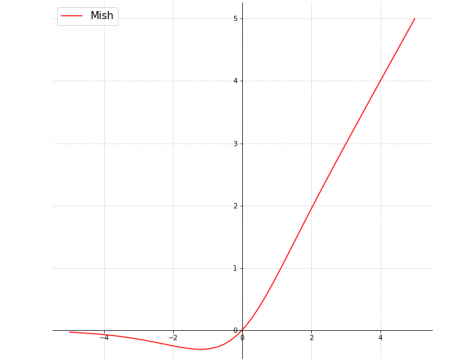
\includegraphics[width=.9\linewidth]{mish.png}
			\end{center}
		\end{column}
		\hfill
		\begin{column}{0.5\textwidth}
			Похожим образом получили функции активации Mish
				\[f(x) = x \cdot tanh(\ln(1 + e^x)) \]
		\end{column}
	\end{columns}
	\vfill %
	\footnotesize
	{\color{blue} \url{https://arxiv.org/pdf/1908.08681.pdf} \newline \url{https://krutikabapat.github.io/Swish-Vs-Mish-Latest-Activation-Functions/} }
\end{frame}


\begin{frame}{Activate or Not, ACON (2020)}
\begin{wideitemize} 
	\item  Swish -- гладкий вариант ReLU с гейтом 
	\item  Функция сама решает, нужна слою активация или нет 
	\item  Можно обобщить этот подход и придумать более интересные функции потерь, которые дадут улучшение
\end{wideitemize}	
\vfill %
\footnotesize
{\color{blue} \url{https://arxiv.org/pdf/2009.04759.pdf}}
\end{frame}


%Подход в общем классический. Давайте поймём как имеющиеся функции можно обобщить, а потом из этого обобщения предложим что-нибудь интересное. Заодно и интуицию обретём.
%
%Логические шаги тут следующие:

%1. Функцию max можно аппроксимировать гладким и дифференцируемым вариантом, который мы будем называть smooth maximum с параметром β, который когда стремится к бесконечности, даёт в пределе максимум, а когда стремится к нулю — арифметическое среднее.
%
%S_β(x_1, ..., x_n) = sum(x_i*exp(β*x_i))/sum(exp(β*x_i))
%
%2. ReLU это, как известно, max(x,0), а значит можно аппроксимировать этим нашим гладким максимумом о двух входах: 
%
%S_β(η_a(x), η_b(x))
%и η_a(x) = x, η_b(x) = 0,
%
%3. Swish тоже можно представить через эту функцию S_β(x, 0) = x * σ(β*x) и её мы называем ACON-A. А заодно Swish — это гладкая аппроксимация ReLU.
%
%4. Если рассмотреть развития ReLU типа PReLU, Leaky ReLU и т.п., то можно прийти к функции ACON-B c n η_a(x) = x, η_b(x) = px.
%
%5. Можно пойти ещё дальше и сделать ACON-C с η_a(x) = p_1*x, η_b(x) = p_2*x(p_1 != p_2). ACON-C в такой формулировке позволяет иметь обучаемые верхние и нижние границы для градиента (у Swish они фиксированы). Они определяются параметрами p_1 и p_2.
%
%6. Ну и наконец параметр β тоже можно обучать и это даёт функцию Meta-ACON. Этот параметр называется switching factor и регулирует поведение нейрона: линейный (неактивный нейрон) или нелинейный режим работы (активный нейрон). Отсюда и название ActivateOrNot (ACON).
%
%И вот эта последняя история открывает целое пространство для исследования, можно реализовывать разные функции, генерящие эту β по входным данным: можно иметь общий параметр на весь слой, можно на отдельные каналы, а можно и на пиксели.
%
%Что вообще даёт вся эта эквилибристика? На редкость неплохие улучшения, единицы процентных пунктов в терминах top-1 ошибки. Для которых от вас по большому счёту ничего не требуется кроме замены функции активации.
%
%Ну и заодно вроде понятнее стало, что такое Swish и вообще.


\begin{frame}{ TLDR: что на практике}
	\begin{wideitemize}
		\item Начните с ReLU, аккуратно инициализируйте веса и настраивайте скорость обучения
		\item Попробуйте Leaky ReLU / ELU / SELU / Swish / Mish, если есть время на эксперименты, чтобы выжать максимум
		\item Не используйте сигмоиду и  tanh
	\end{wideitemize}
\vfill %
\footnotesize
Краткий обзор функций активаций: {\color{blue}  \url{https://arxiv.org/pdf/1804.02763.pdf}}
\end{frame}


\begin{transitionframe}
	\begin{center}
		\Huge  Предобработка данных
	\end{center}
\centering \includegraphics[scale = 0.2]{prepare.png}
\end{transitionframe}


\begin{frame}{Предобработка данных}
\begin{center}
	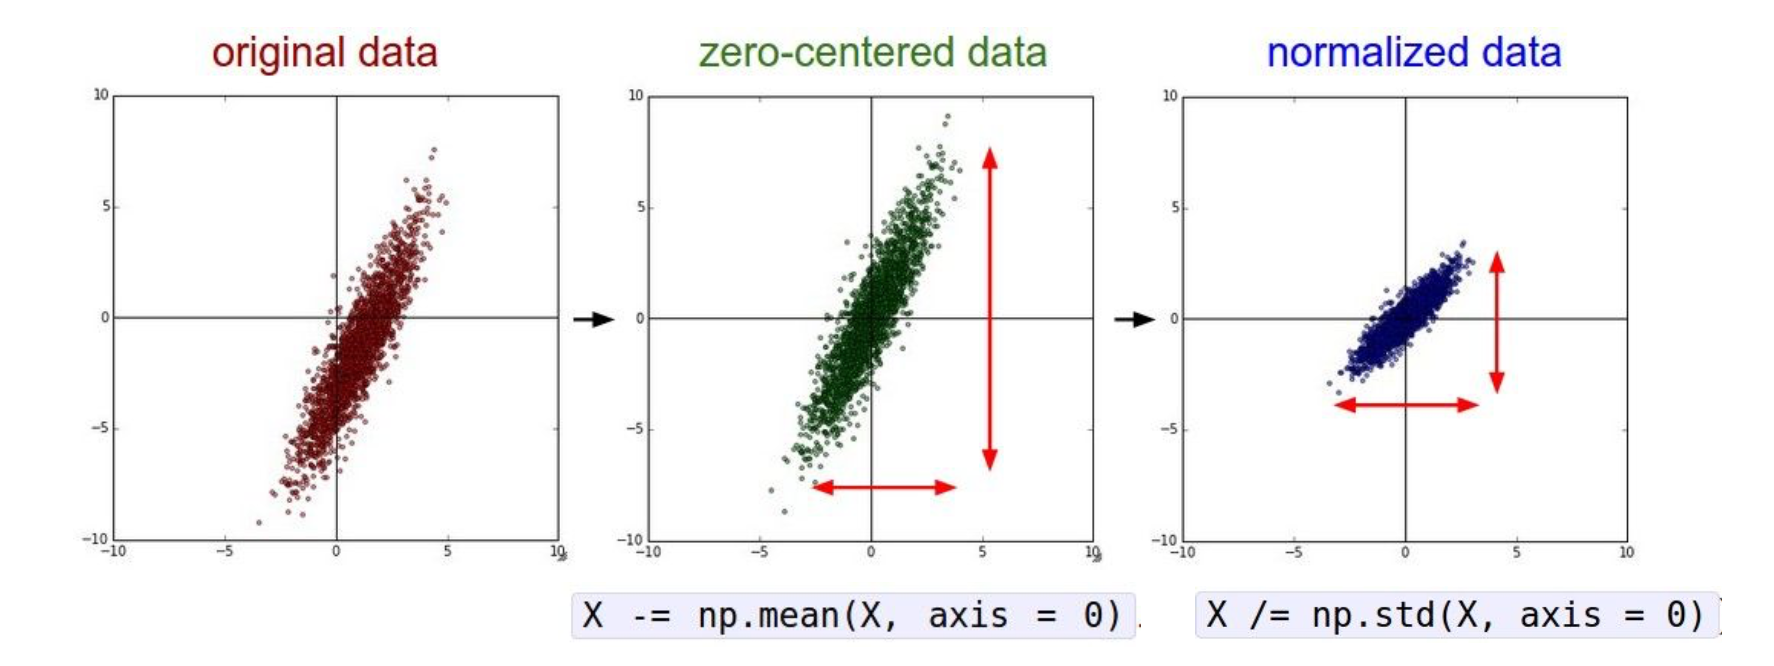
\includegraphics[width=0.99\paperwidth]{data_norm.png}
\end{center}
\vfill %
\footnotesize
{\color{blue}  \url{http://cs231n.stanford.edu/slides/2021/}}
\end{frame}


\begin{frame}{Предобработка табличных данных}
	\begin{columns}
	\begin{column}{0.5\textwidth}
		\alert{Без нормализации}
		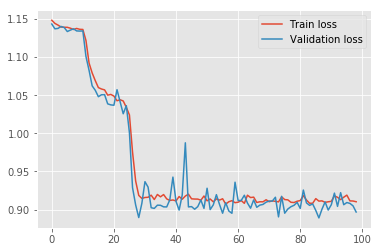
\includegraphics[width=.95\linewidth]{no_prep.png}
	\end{column}
	\hfill
	\begin{column}{0.5\textwidth}
		\alert{С нормализацией}
		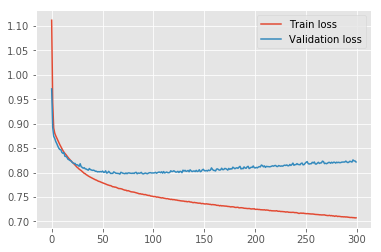
\includegraphics[width=.95\linewidth]{with_prep.png}
	\end{column}
\end{columns}
\end{frame}


\begin{frame}{Зачем нормализация картинкам?}
\begin{columns}
	\begin{column}{0.6\textwidth}
			\begin{wideitemize}
			\item \alert{Что происходит, когда все входы в нейрон положительные?}
			\item Все градиенты либо положительные либо отрицательные 
			\item Картинки центрируют для того, чтобы были отрицательные входы
			\item Картинки нормируют, чтобы инициализированным в окрестности нуля весам легче было сходиться
		\end{wideitemize}
	\end{column}
	\hfill
	\begin{column}{0.4\textwidth}
		
		\begin{center}
			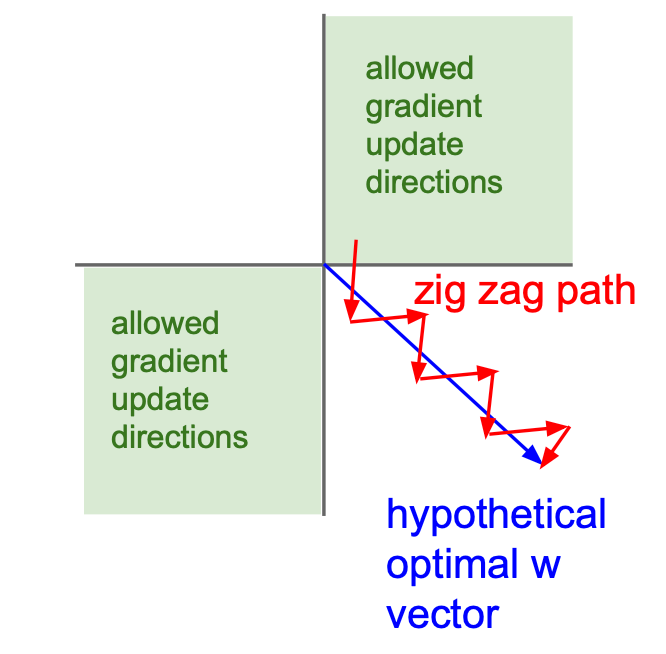
\includegraphics[width=0.98\textwidth]{gr_update.png} 
		\end{center} 
	\end{column}
\end{columns}
\end{frame}


\begin{transitionframe}
	\begin{center}
		\Huge  Инициализация весов
	\end{center}
	\centering 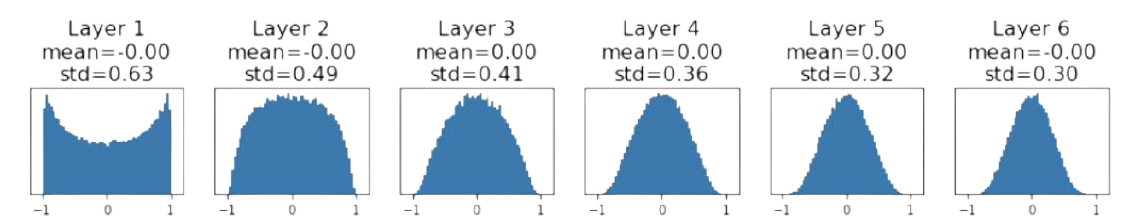
\includegraphics[width=.8\linewidth]{glorot_init_hist-removebg-preview.png}
\end{transitionframe}


\begin{frame}{Инициализация весов}
	\begin{center}
		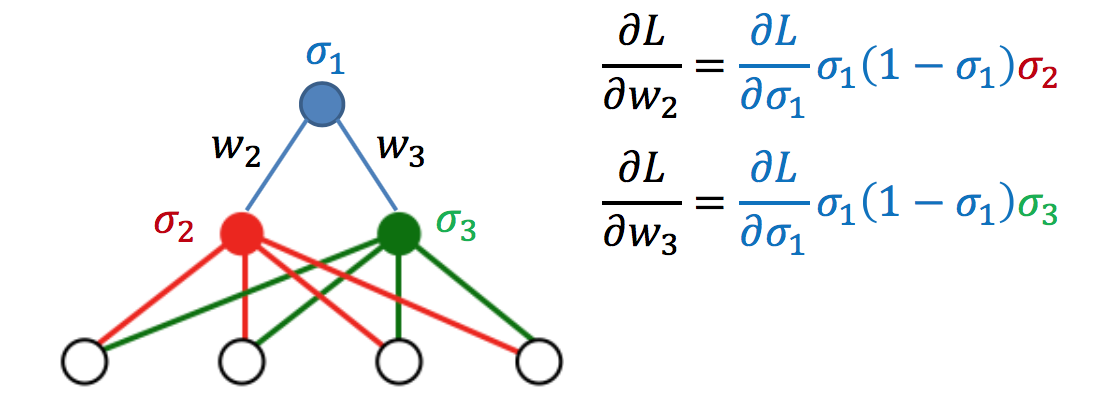
\includegraphics[width=.6\linewidth]{init1.png}
	\end{center}
	\begin{wideitemize}
		\item  Что будет, если инициализировать веса нулями?  \pause 
		\item  ${\color{red} \sigma_2 }$ и ${\color{green} \sigma_3 }$  будут обновляться одинаково
	\end{wideitemize}
\end{frame}


\begin{frame}{Инициализация весов}
	\begin{center}
		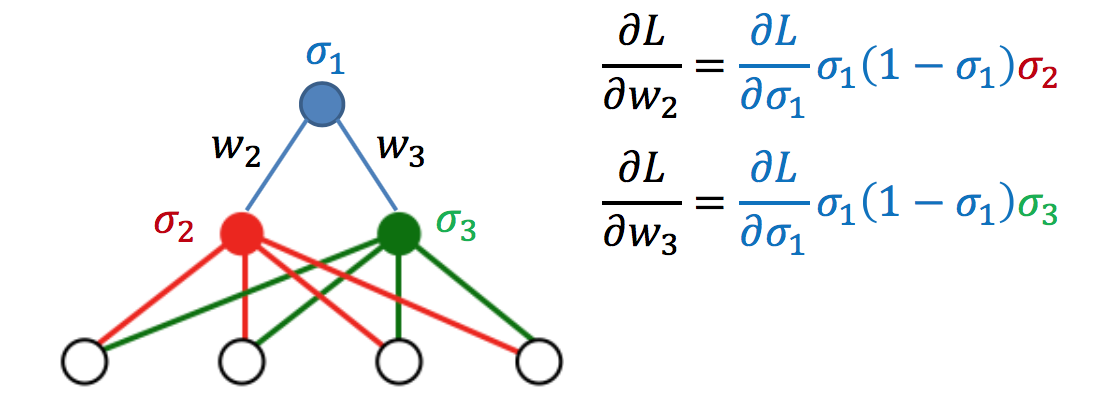
\includegraphics[width=.6\linewidth]{init1.png}
	\end{center}
	\begin{wideitemize}
		\item  Хочется уничтожить симметрию
		\item  Можно инициализировать маленькими рандомными числами из какого-то распределения (нормальное, равномерное)
		\item {\color{red}  Это будет плохо работать для глубоких сетей} 
	\end{wideitemize}
\end{frame}


% Тут мне пиздец было влом настраивать minted и я упоролся
\begin{frame}{Инициализация весов}
\begin{columns}
	\begin{column}{.45\textwidth}
		\only<1-2>{		
		\begin{wideitemize} 
		 \item Прямой проход через 6 слоёв нейросети
		 \item \alert{Что произойдёт с активацией к последнему слою?}
		 \only<2>{\item Активация постепенно стягивается к нулю }
		\end{wideitemize}}
	\only<3-4>{
	\begin{wideitemize} 
			\item Активация постепенно стягивается к нулю
			\item \alert{А что будет происходить с градиентами?}
			\only<4>{\item Все будут нулевыми :(  }
	\end{wideitemize}}
	\end{column}
	\begin{column}{.55\textwidth}
		dims = [{\color{green} 4096}] *  {\color{green} 7} \\
		hs = [ ] \\
		x = np.random.randn(  {\color{green} 16}, dims[  {\color{green} 0} ]) \\
		{\color{green} for} Din, Dout {\color{green} in zip}(dims[:  {\color{green} -1}], dims[ {\color{green} 1}:]): \\  
		\mbox{ } \hspace{5mm} W =  {\color{green} 0.01} * np.random.randn(Din, Dout) \\
		\mbox{ } \hspace{5mm} x = np.tanh(x.dot(W)) \\
		\mbox{ } \hspace{5mm} hs.append(x)
	\end{column}
\end{columns}
\hfill \only<2->{
\begin{center}
	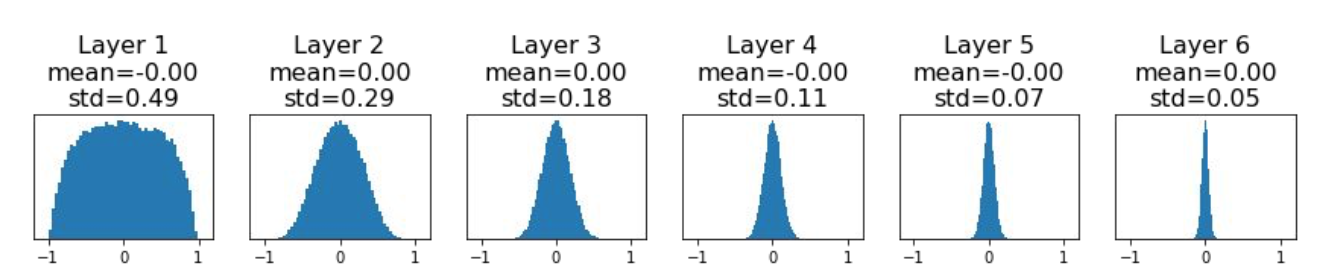
\includegraphics[width=.99\linewidth]{init_tanh_activation.png}
\end{center}}
\end{frame}


\begin{frame}{Инициализация весов}
\begin{columns}
	\begin{column}{.45\textwidth}
		\only<1-2>{		
			\begin{wideitemize} 
				\only<1>{\item Увеличим стандартное отклонение в инициализации с $0.01$ до $0.05$
				\item \alert{Что произойдёт с активацией к последнему слою?}}
				\only<2>{\item Постепенно происходит насыщение, \alert{градиенты опять занулятся} }
		\end{wideitemize}}
	\end{column}
	\begin{column}{.55\textwidth}
		dims = [{\color{green} 4096}] *  {\color{green} 7} \\
		hs = [ ] \\
		x = np.random.randn(  {\color{green} 16}, dims[  {\color{green} 0} ]) \\
		{\color{green} for} Din, Dout {\color{green} in zip}(dims[:  {\color{green} -1}], dims[ {\color{green} 1}:]): \\  
		\mbox{ } \hspace{5mm} W =  {\color{red} \textbf {0.05} } * np.random.randn(Din, Dout) \\
		\mbox{ } \hspace{5mm} x = np.tanh(x.dot(W)) \\
		\mbox{ } \hspace{5mm} hs.append(x)
	\end{column}
\end{columns}
\hfill \only<2->{
	\begin{center}
		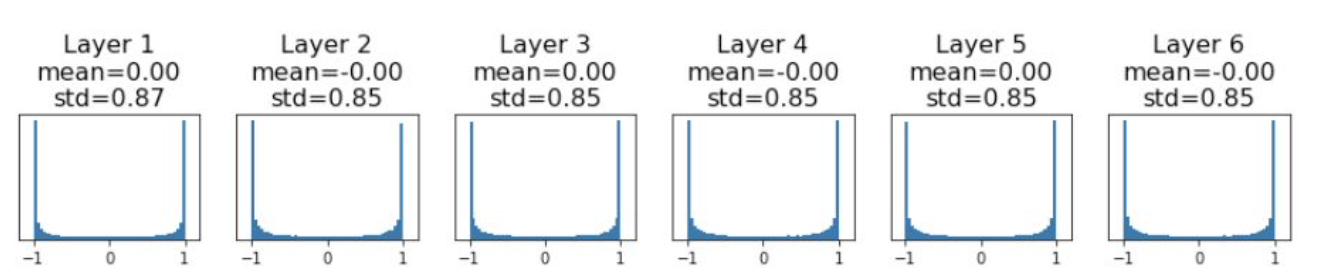
\includegraphics[width=.99\linewidth]{bad_init_tanh.png}
\end{center}}
\end{frame}


\begin{frame}{Инициализация весов}
\begin{columns}
	\begin{column}{.3\textwidth}	
			\begin{wideitemize} 
				\item Распределение активаций не меняется,  \alert{с градиентами всё хорошо}
		\end{wideitemize}
	\end{column}
	\begin{column}{.7\textwidth}
		dims = [{\color{green} 4096}] *  {\color{green} 7} \\
		hs = [ ] \\
		x = np.random.randn(  {\color{green} 16}, dims[  {\color{green} 0} ]) \\
		{\color{green} for} Din, Dout {\color{green} in zip}(dims[:  {\color{green} -1}], dims[ {\color{green} 1}:]): \\  
		\mbox{ } \hspace{5mm} W =  {\color{red} \textbf {1/np.sqrt(Din)} } * np.random.randn(Din, Dout) \\
		\mbox{ } \hspace{5mm} x = np.tanh(x.dot(W)) \\
		\mbox{ } \hspace{5mm} hs.append(x)
	\end{column}
\end{columns}
	\begin{center}
		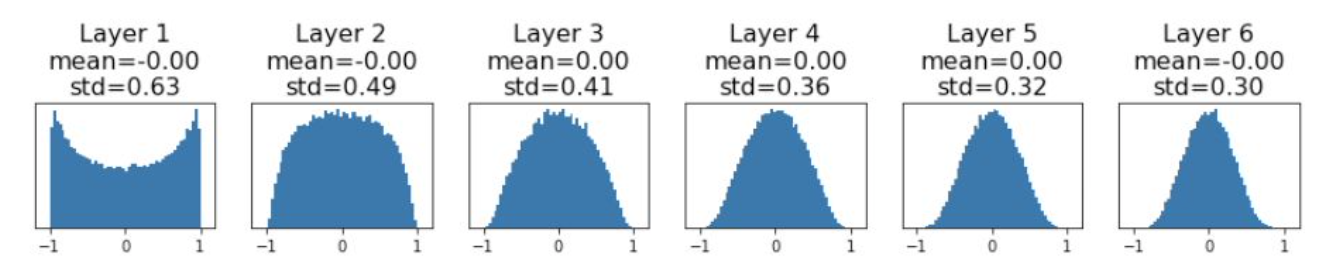
\includegraphics[width=.99\linewidth]{glorot_init_hist.png}
\end{center}
\end{frame}


\begin{frame}{Инициализация весов}
	\begin{wideitemize}
		\item  Посмотрим на выход нейрона перед активацией:
	\begin{equation*}
		\begin{aligned} 
			h_i =  \sum_{i=1}^{n_{in}} w_i x_i 
		\end{aligned}
	\end{equation*}
		\item  Дисперсия $h_i$ выражается через дисперсии $x$ и $w$ 
		\item Будем считать, что веса $w_1, \ldots, w_k \sim iid$,  наблюдения $x_1, \ldots, x_n \sim iid$, а ещё $x_i$ и $w_i$ независимы между собой
	\end{wideitemize}
\end{frame}


\begin{frame}{Инициализация весов (симметричная активация)}
\begin{multline*} 	
\Var(h_i) = \Var(\sum_{i=1}^{n_{in}} w_i x_i) =  \sum_{i=1}^{n_{in}} \Var(w_i x_i) = \\ 
= \sum_{i=1}^{n_{in}} [\E(x_i)]^2 \cdot \Var(w_i) + [\E(w_i)]^2 \cdot \Var(x_i)  + \Var(x_i) \cdot \Var(w_i)] = \only<3->{\\  =  \sum_{i=1}^{n_{in}}  \Var(x_i) \cdot \Var(w_i)  } \only<4>{ =  \Var(x)  \color{green} \cdot [n_{in} \cdot \Var(w)]} \only<5->{ =  \Var(x)  \color{green} \cdot \underbrace{[n_{in} \cdot \Var(w)]}_{= 1}}
\end{multline*}
\only<2-4>{

\begin{wideitemize}
\only<2>{ \item  Если функция активации симметричная, тогда $E(x_i) = 0$. Будем инициализировать веса с нулевым средним, тогда $E(w_i) = 0$.}

\only<3>{ 
\item  Предполагаем, что $x_i$ инициализируются из одного распределения, $w_i$ сами инициализируем из одного распределения.}

\only<4>{ 
\item  Хотим, чтобы зелёная штука была равна единице, тогда у потока будет всегда постоянная дисперсия, совпадающая с $\Var(x)$.}
\end{wideitemize}}

\only<1>{
\vfill %
\footnotesize
{\color{blue}  \url{https://en.wikipedia.org/wiki/Variance\#Product\_of\_independent\_variables}}}
\end{frame}


\begin{frame}{Плохая инициализация весов}
	Пусть
	
	$$ w_i \sim U \left[ - \frac{1}{\sqrt{n_{in}}};  \frac{1}{\sqrt{n_{in}}}  \right],$$
	
	тогда 
	
	$$
	\Var(w_i) = \frac{1}{12} \cdot \left( \frac{1}{\sqrt{n_{in}}} + \frac{1}{\sqrt{n_{in}}} \right)^2 = \frac{1}{3 n_{in}} \Rightarrow Var(h_i) = \frac{1}{3} 
	$$
	
	\alert{Получаем затухание!}
\end{frame}


\begin{frame}{Инициализация Ксавье/Глорота (2010)}
	Пусть
	
	$$ w_i \sim U \left[ - \frac{\sqrt{3}}{\sqrt{n_{in}}};  \frac{\sqrt{3}}{\sqrt{n_{in}}}  \right],$$
	
	тогда 
	
	$$
	\Var(w_i) = \frac{1}{12} \cdot \left( \frac{\sqrt{3}}{\sqrt{n_{in}}} + \frac{\sqrt{3}}{\sqrt{n_{in}}} \right)^2 = \frac{1}{n_{in}} \Rightarrow Var(h_i) = 1 \pause 
	$$
	
	\vfill 
	При forward pass на вход идёт $n_{in}$ наблюдений, при backward pass на вход идёт $n_{out}$ градиентов $\Rightarrow$   \alert{канал с дисперсией может быть непостоянным, если число весов от слоя к слою сильно колеблется}
\end{frame}


\begin{frame}{Инициализация Ксавье/Глорота (2010)}
	\begin{wideitemize}
		\item Для неодинаковых размеров слоёв невозможно удовлетворить обоим условиям, поэтому обычно усредняют и пытаются инициализировать веса с дисперсией $$\frac{2}{n_{in} + n_{out}}$$
		
		\item Такая инициализация называется \alert{инициализацией Ксавие (или Глорота)}
	
		$$ w_i \sim U \left[ - \frac{\sqrt{6}}{\sqrt{n_{out} + n_{in}}};  \frac{\sqrt{6}}{\sqrt{n_{out} + n_{in}}}  \right],$$
		
	\end{wideitemize}
	\vfill %
	\footnotesize
	{\color{blue} \url{http://proceedings.mlr.press/v9/glorot10a/glorot10a.pdf}}
\end{frame}


\begin{frame}{А что с ReLU?}
	\begin{columns}
	\begin{column}{.3\textwidth}	
		Инициализация Ксавье предполагает симметричную функцию активации
	\end{column}
	\begin{column}{.7\textwidth}
		dims = [{\color{green} 4096}] *  {\color{green} 7} \\
		hs = [ ] \\
		x = np.random.randn(  {\color{green} 16}, dims[  {\color{green} 0} ]) \\
		{\color{green} for} Din, Dout {\color{green} in zip}(dims[:  {\color{green} -1}], dims[ {\color{green} 1}:]): \\  
		\mbox{ } \hspace{5mm} W =  1/np.sqrt(Din) * np.random.randn(Din, Dout) \\
		\mbox{ } \hspace{5mm} {\color{red} \textbf {x = np.max(0, x.dot(W))} } \\
		\mbox{ } \hspace{5mm} hs.append(x)
	\end{column}
\end{columns}
\begin{center}
	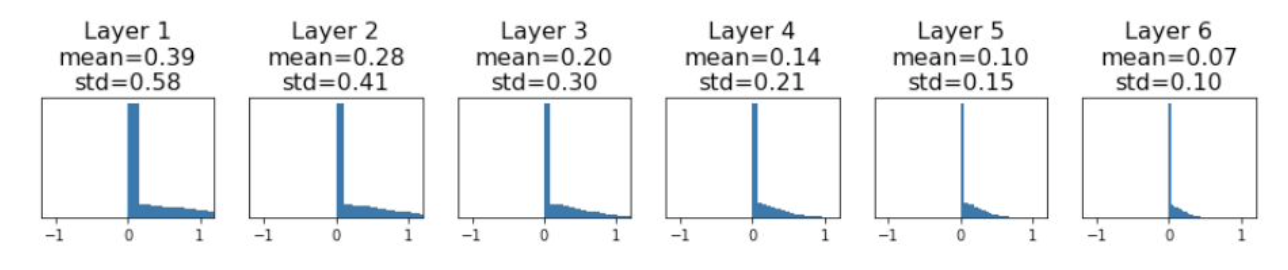
\includegraphics[width=.99\linewidth]{relu_init_x.png}
\end{center}
\end{frame}


\begin{frame}{А что с ReLU?}
\begin{columns}
	\begin{column}{.3\textwidth}	
		Инициализация Ксавье предполагает симметричную функцию активации
	\end{column}
	\begin{column}{.7\textwidth}
		dims = [{\color{green} 4096}] *  {\color{green} 7} \\
		hs = [ ] \\
		x = np.random.randn(  {\color{green} 16}, dims[  {\color{green} 0} ]) \\
		{\color{green} for} Din, Dout {\color{green} in zip}(dims[:  {\color{green} -1}], dims[ {\color{green} 1}:]): \\  
		\mbox{ } \hspace{5mm} W =  {\color{red} \textbf {np.sqrt(2/Din)} } * np.random.randn(Din, Dout) \\
		\mbox{ } \hspace{5mm} {\color{red} \textbf {x = np.max(0, x.dot(W))} } \\
		\mbox{ } \hspace{5mm} hs.append(x)
	\end{column}
\end{columns}
\begin{center}
	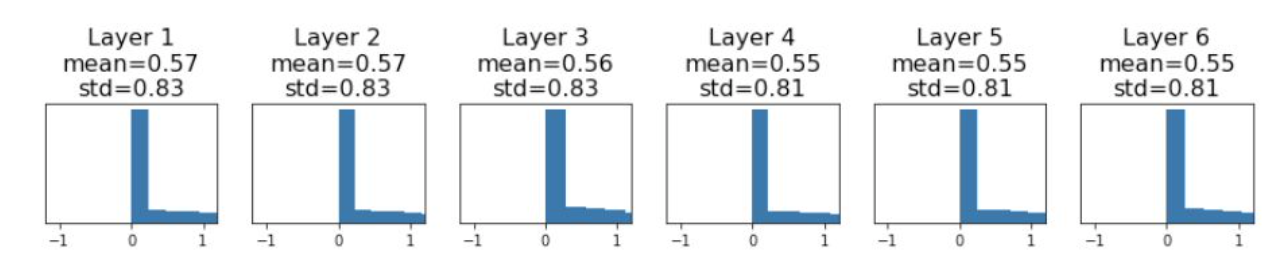
\includegraphics[width=.99\linewidth]{relu_init_xe.png}
\end{center}
\end{frame}



\begin{frame}{Инициализация Хе (2015)}
	\begin{multline*} 	
		\Var(h_i) = \Var(\sum_{i=1}^{n_{in}} w_i x_i) =  \sum_{i=1}^{n_{in}} \Var(w_i x_i) = \\ 
		= \sum_{i=1}^{n_{in}} [\E(x_i)]^2 \cdot \Var(w_i) + [\E(w_i)]^2 \cdot \Var(x_i)  + \Var(x_i) \cdot \Var(w_i)]  
		\only<2->{= \\  = \sum_{i=1}^{n_{in}} [\E(x_i)]^2 \cdot \Var(w_i) +  \Var(x_i) \cdot \Var(w_i)  =  \sum_{i=1}^{n_{in}} \Var(w_i) \cdot E(x_i^2)} 
		\only<3->{= \\  =  E(x^2)  \color{green} \cdot [n_{in} \cdot \Var(w)]}
	\end{multline*}

	\only<1-2>{	
	\begin{wideitemize}
		\item  Когда нет симметрии, можно занулить только второе слагаемое
	\end{wideitemize}}
\end{frame}


\begin{frame}{Инициализация Хе (2015)}
	\begin{align*} 	
		\Var(h_i)  & =   E(x_i^2)  \cdot [n_{in} \cdot \Var(w)] \\
	x_i & = \max(0; h_{i-1}) \\ 
	\end{align*} \pause 

	\only<2-> { Пусть $w_{i-1}$ распределены симметрично относительно нуля, тогда $h_{i-1}$ тоже будут симметрично распределены, тогда: }

	$$
	\only<3->{ E(x_i^2) = \frac{1}{2} \cdot \Var(h_{i-1}) }
	$$

	$$
	\only<4->{ \Var(h_i) =  \frac{1}{2} \cdot \Var(h_{i-1}) \cdot [n_{in} \cdot \Var(w)]  \Rightarrow \Var(w_i) = \frac{2}{n_{in}} }
	$$

	\vfill %
	\footnotesize
	{\color{blue} \url{https://arxiv.org/pdf/1502.01852.pdf}}
\end{frame}


\begin{frame}{TLDR: что на практике}
	\begin{wideitemize}
		\item  Для симметричных функций с нулевым средним используйте инициализацию Ксавье (Глорота) {\color{green}  init="glorot\_uniform"} 
		\item  Для ReLU и им подобным инициализацию Хe {\color{green} init="he\_uniform"} или {\color{green} init="he\_nomal"}
		\item  Эти две инициализации корректируют параметры распределений в зависимости от входа и выхода слоя так, чтобы поддерживать дисперсию равной единице
	\end{wideitemize}
\end{frame}


\begin{frame}{Тема инициализации сегодня активно исследуется}
\scriptsize{
	\begin{wideitemize} 
	\item Understanding the difficulty of training deep feedforward neural networks
	by Glorot and Bengio, 2010 
	
	\item Exact solutions to the nonlinear dynamics of learning in deep linear neural networks by Saxe et al, 2013 
	
	\item Random walk initialization for training very deep feedforward networks by Sussillo and Abbott, 2014 
	
	\item Delving deep into rectifiers: Surpassing human-level performance on ImageNet classification by He et al., 2015 
	
	\item Data-dependent Initializations of Convolutional Neural Networks by Krähenbühl et al., 2015 
	
	\item All you need is a good init, Mishkin and Matas, 2015 
	
	\item Fixup Initialization: Residual Learning Without Normalization, Zhang et al, 2019 
	
	\item The Lottery Ticket Hypothesis: Finding Sparse, Trainable Neural Networks, Frankle and Carbin, 2019
	\end{wideitemize}}
\end{frame}


\begin{transitionframe}
	\begin{center}
		\Huge Переобучение нейронных сетей
	\end{center}
	\centering 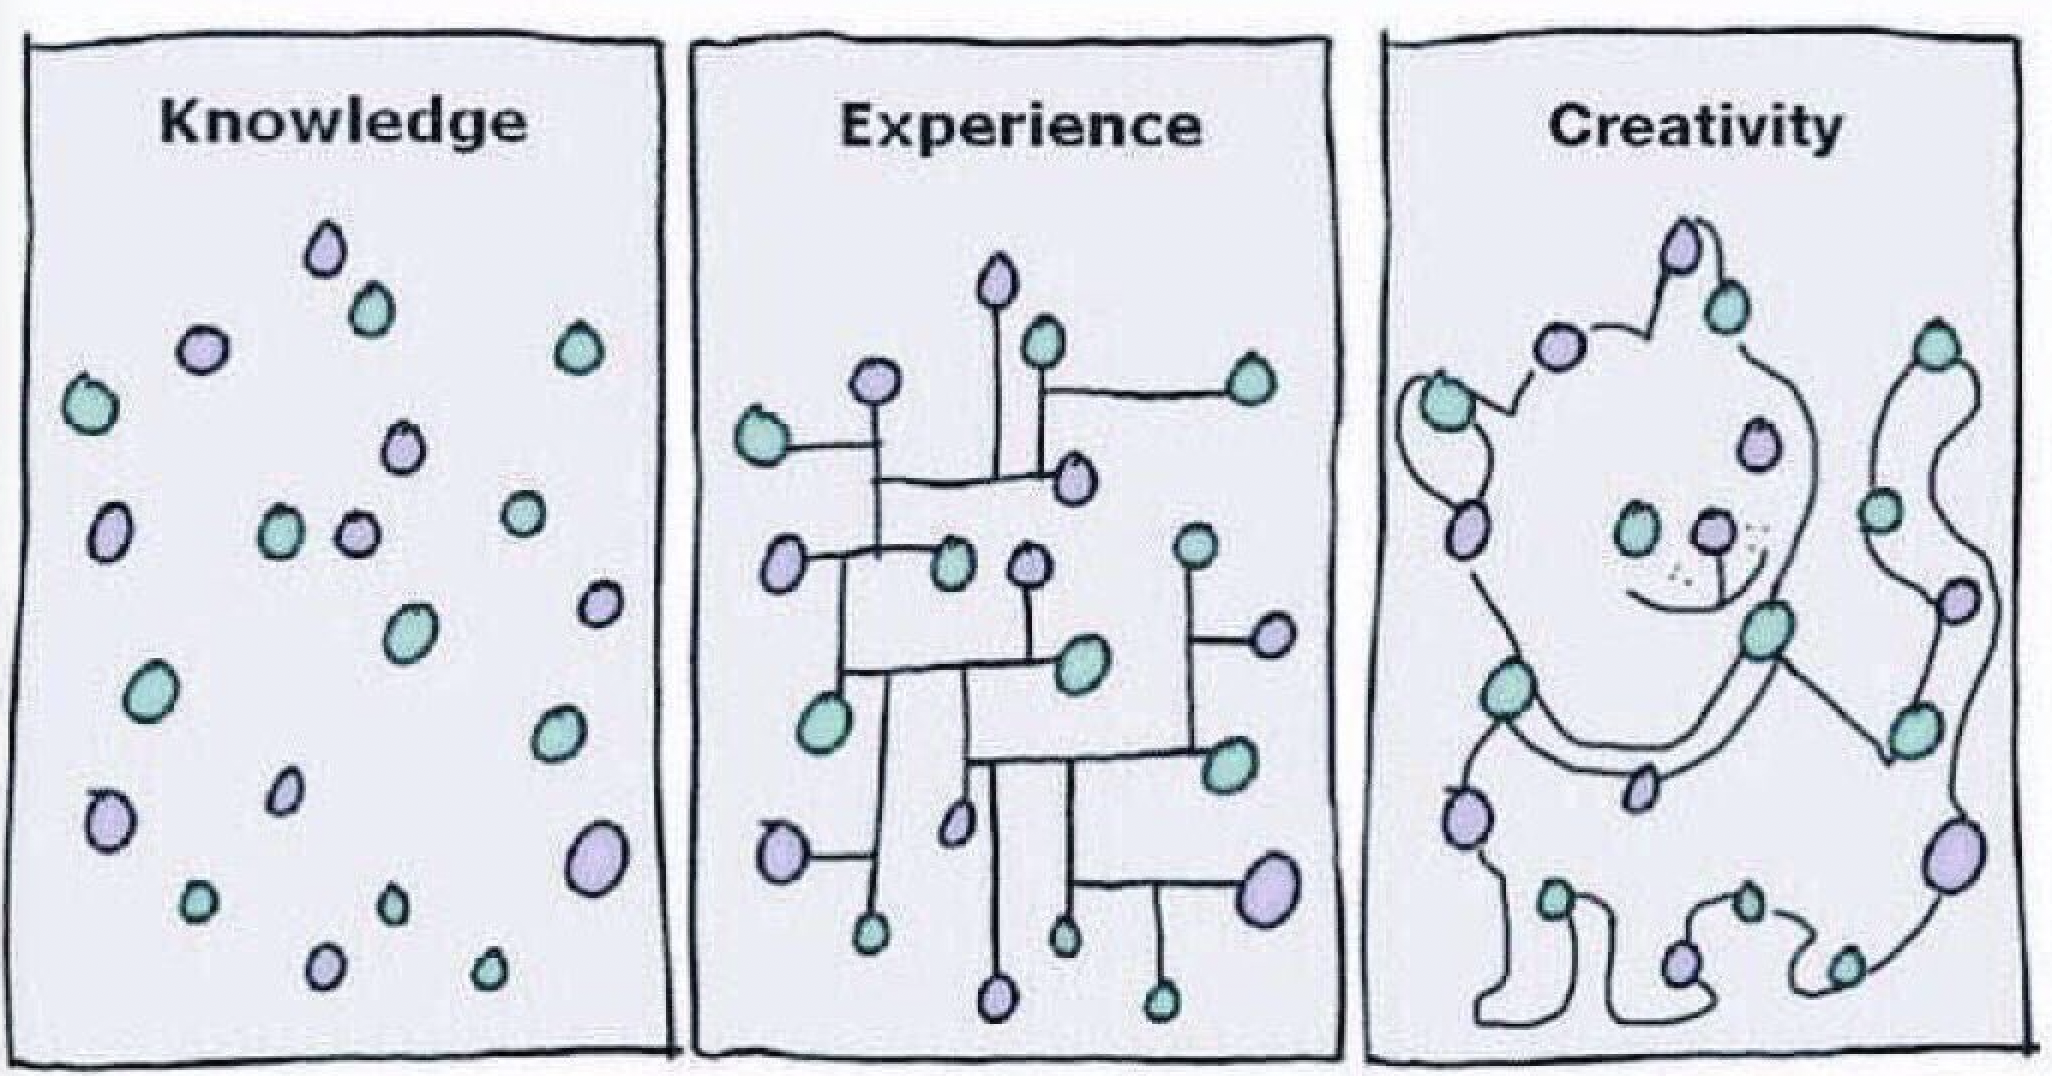
\includegraphics[scale = 0.2]{over.png}
\end{transitionframe}


\begin{frame}{Что такое асимптотика?}
	\begin{wideitemize}
		\item $n$ — число наблюдений  \only<3-4>{$k$ — число параметров}
		\item Обучение почти любой ML-модели  — максимизация правдоподобия 
		\item \only<1>{ При $n \to \infty$ модель работает хорошо} \only<2-4>{\sout{При $n \to \infty$ модель работает хорошо}}
		\only<3-4>{\item \alert{При $\frac{n}{k} \to \infty$ модель работает хорошо}}
		\only<4>{\item Мы живём в эпоху перепараметризованных моделей, $k >> n$ }
		\only<4>{\item У таких моделей вскрывается много интересных свойств}
	\end{wideitemize}
\end{frame}


{
	\usebackgroundtemplate{ 
		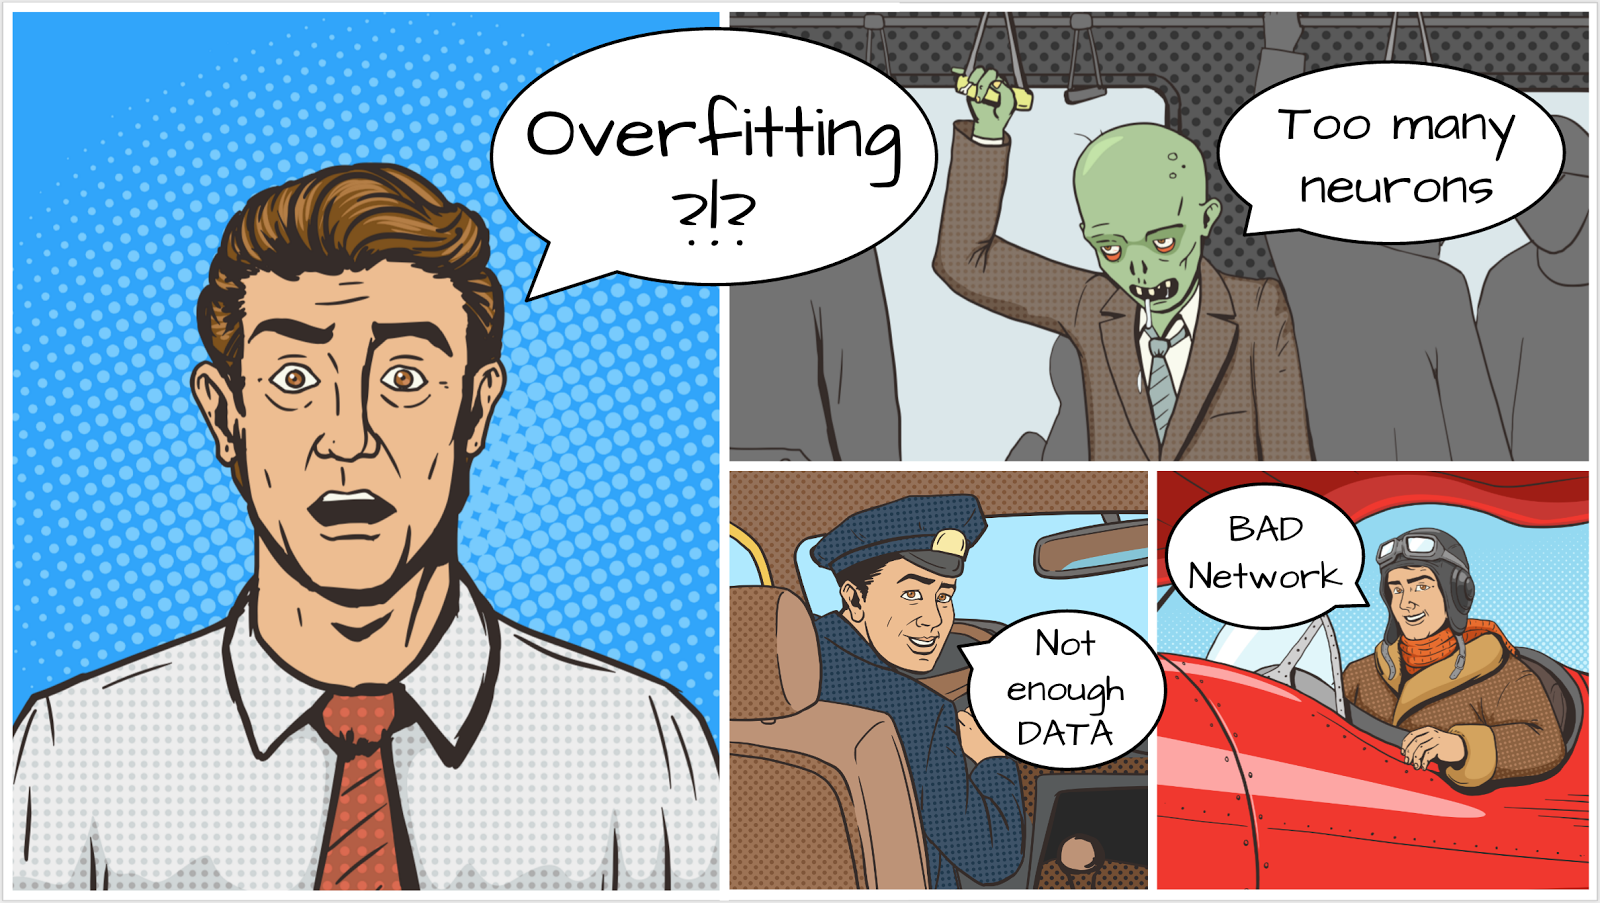
\includegraphics[width=\paperwidth]{overfitting.png}}
	\begin{frame}
\end{frame}
}


\begin{frame}{Размеры сеток и переобучение}
	\begin{center}
		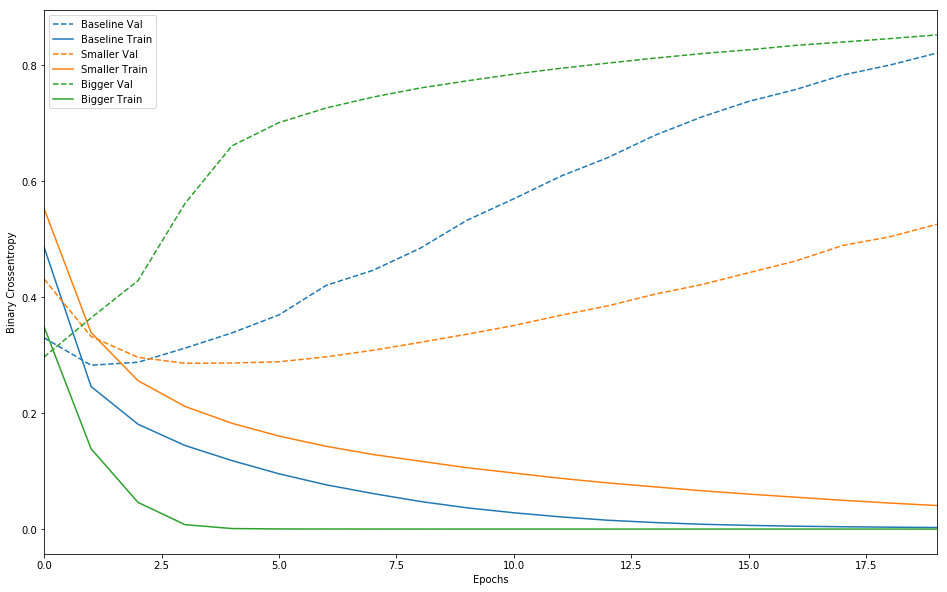
\includegraphics[width=0.7\paperwidth]{big_base_small_fit.png}
	\end{center}
\end{frame}


\begin{frame}{Борьба с переобучением}
	\begin{wideitemize}
		\item Граница сильно размыта
		\item Сокращение числа параметров, изобретение более эффективных архитектур
		\item Регуляризация, разные способы мешать модели подгоняться под обучающую выборку
		\item Более эффективные методы оптимизации
	\end{wideitemize}
\end{frame}


\begin{frame}{Регуляризация}
\begin{wideitemize}
	\item $L_2$: приплюсовываем к функции потерь $\lambda \cdot \sum w_i^2$
	
	\item $L_1$: приплюсовываем к функции потерь $\lambda \cdot \sum |w_i|$
	
	\item Можно регуляризовать не всю сетку, а отдельный нейрон или слой
	
	\item Можно наложить регуляризацию на выход из слоя
	
	\item Не даёт нейрону сфокусироваться на слишком выделяющемся входе	
	
	\item Любой дополнительный шум в данных — регуляризация
\end{wideitemize}
\end{frame}


\begin{frame}{Ранняя остановка (early stopping)}
\begin{center}
	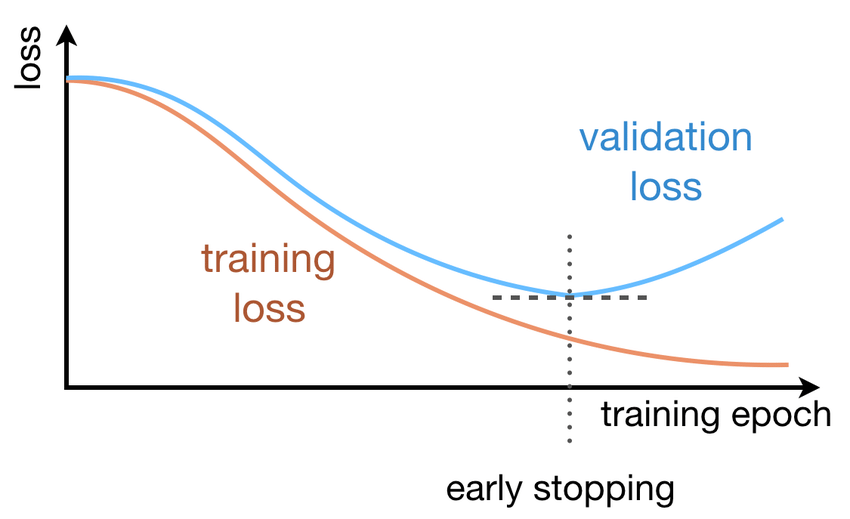
\includegraphics[width=.95\linewidth]{early_stopping.png}
\end{center}
\end{frame}


\begin{frame}{Ранняя остановка (early stopping)}
\begin{wideitemize}
	\item  Будем останавливать обучение, когда качество на валидации начинает падать
	\item  Ранняя остановка действует примерно также, как регуляризаторы 
	\item  Например, в книге  Гудфеллоу "Глубокое обучение" на стр. 218 можно найти, что ранняя остановка для линейных моделей эквивалентна $l_2$ регуляризации с MSE, обучаемой SGD
\end{wideitemize}
\end{frame}


\begin{frame}{Ругуляризация и Dropout}
\begin{wideitemize}
	\item  На практике обычно используют Dropout
	
	\item Он работает похожим на регуляризаторы образом
	
	\item Например, в [1] написано: \\ \mbox{   } \\
	
	\texttt{«We show that the dropout regularizer is first-order equivalent to an L2 regularizer applied after scaling the features by an estimate of the inverse diagonal Fisher information matrix»}
\end{wideitemize}
\vfill %
\footnotesize 
\color{blue} [1] \url{https://arxiv.org/abs/1307.1493} 
\end{frame}


\begin{transitionframe}
	\begin{center}
		% \Huge Dropout  
		
\includegraphics[scale = 0.25]{dropout_beer.png}
	\end{center}
\end{transitionframe}


% Оформить слайд как цитату, мб впихнуть фотку Хинтона
\begin{frame}{Хинтон и банк}

 Посещая свой банк я заметил, что операционисты, обслуживающие меня, часто меняются. Я спросил одного из них, почему так происходит. Он сказал, что не знает, но им часто приходится переходить с места на место. Я предположил, что это делается для исключения мошеннического сговора с сотрудником банка. 
 
 \par \mbox{ } \par 
 
  Это навело меня на мысль, что \alert{удаление случайно выбранного подмножества нейронов}  из каждого примера может помочь \alert{предотвратить заговор модели с исходными данными} и ослабить эффект переобучения. 

\vfill %
\footnotesize
{\color{blue} \url{https://www.reddit.com/r/MachineLearning/comments/4w6tsv/ama_we_are_the_google_brain_team_wed_love_to}}
\end{frame}


\begin{frame}{Dropout}
\begin{wideitemize}	
	\item При каждом прямом проходе мы зануляем выход нейрона с вероятностью $p$ 
	\item Делает нейроны более устойчивыми к случайным возмущениям
\end{wideitemize}

\begin{center}
	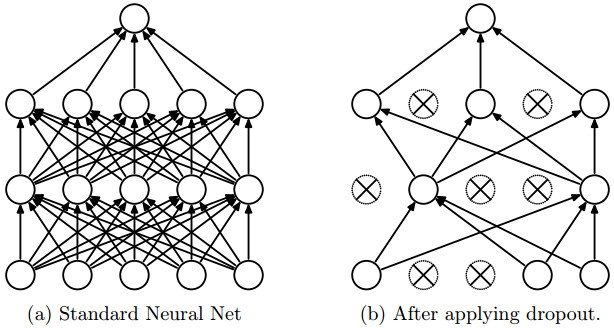
\includegraphics[width=0.5\paperwidth]{dropout2.png}
\end{center}

\vfill %
\footnotesize
{\color{blue} \url{http://www.cs.toronto.edu/~rsalakhu/papers/srivastava14a.pdf}}
\end{frame}


\begin{frame}{Dropout}
\begin{wideitemize}	
		\item Борьба с ко-адоптацией, не все соседи похожи  друг на друга, не все дети похожи  на родителей
		\item  Dropout эквивалентен обучению ансамбля из $2^n$ сетей
\end{wideitemize}

\begin{center}
	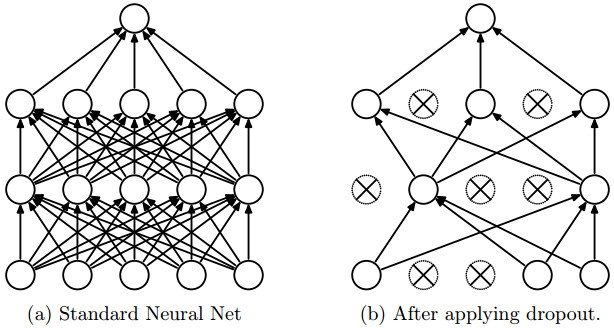
\includegraphics[width=0.5\paperwidth]{dropout2.png}
\end{center}

\vfill %
\footnotesize
{\color{blue} \url{http://www.cs.toronto.edu/~rsalakhu/papers/srivastava14a.pdf}}
\end{frame}


\begin{frame}{Dropout в формулах} 
	\begin{wideitemize}
		\item  Можно определить как слой $d(h)$ 
		\item  Параметров у слоя нет, есть только гиперпараметр $p$
		\pause 
		\item  	forward pass без dropout:  \[o = f(XW)\]
		\item  	forward pass с dropout:  \[o = d \cdot f(XW), \quad d = (d_1, \ldots, d_k)  \sim iid \vspace{5mm} Bern(p)\]
		\pause 	
	\end{wideitemize}
		\[
		o_i = d_i \cdot f(w x_i^T) = \begin{cases} f(w x_i^T) , 1-p \\ 0, p \end{cases}
		\]	
	\vfill 
	\alert{Дропаут — это просто небольшая модификация функции активации}
\end{frame}


\begin{frame}{Dropout в формулах} 
	\begin{wideitemize}
		\item forward pass:
		
		\begin{equation*}
			\begin{aligned}
			& o = f(X \cdot W  ) \\
			& \alert{o = d \cdot f(X \cdot W ), \quad  d = (d_1, \ldots, d_k) \sim iid \vspace{5mm} Bern(p)} 
			\end{aligned}
		\end{equation*}
		
		\item backward pass:
		\begin{equation*}
			\begin{aligned}
			& grad = f'(h) \cdot W \cdot grad  \\
			& \alert{ grad =  d \cdot f'(h) \cdot W \cdot grad} 
			\end{aligned}
		\end{equation*}			
	\end{wideitemize}
\end{frame}


\begin{frame}{Dropout}
\begin{wideitemize}
\item  При обучении мы домножаем часть выходов на $d_i$, тем самым мы изменяем только часть параметров и нейроны учатся более независимо  \alert{$\Rightarrow$ регуляризация}

\item Дропаут выплёвывает случайные выходы,  \alert{ что делать на стадии тестирования?}

 \only<2->{
\item Нам надо сымитировать работу такого ансамбля: можно отключать по очереди все возможные комбинации нейронов, получить $2^n$ прогнозов и усреднить их }

 \only<3->{ \item Но лучше просто брать по дропауту математическое ожидание: 

$$
o = p \cdot f(X \cdot W)
$$}
\end{wideitemize}
\end{frame}

\begin{frame}{Dropout на тестовой выборке}
	\begin{wideitemize}
	\item Но лучше просто брать по дропауту математическое ожидание: 
	
	$$
	o = p \cdot f(X \cdot W)
	$$
	\end{wideitemize}
	\begin{columns}
		\begin{column}{.25\textwidth}
			\begin{center}
				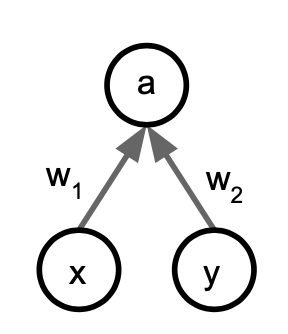
\includegraphics[width=.85\linewidth]{dropout_ex.png}
			\end{center}
		\end{column}
		\begin{column}{.75\textwidth}
			\textbf{Пример:} используем дропаут с вероятностью $0.5$: \\
			\begin{multline*}
				\mathbb{E}(a) = \frac{1}{4} \cdot(w_1 x+ w_2 y) + \frac{1}{4} \cdot(w_1 x+ 0 y) + \\ + \frac{1}{4} \cdot(0 x+ w_2 y) + \frac{1}{4} \cdot(0 x+ 0 y) = \frac{1}{2} \cdot (w_1 \cdot x + w_2 \cdot y)
			\end{multline*}
		\alert{Достаточно домножить выход на $0.5$}
		\end{column}
	\end{columns}
\end{frame}


\begin{frame}{Обратный Dropout}
\begin{wideitemize}
	\item   На тесте ищем математическое ожидание: 
		\[
		o = p \cdot f(X \cdot W )
		\] 
		
	\item \alert{Это неудобно! Надо переписывать функцию для прогнозов!}  \pause
	
	\item Давайте лучше будем домножать на $\frac{1}{p}$ на этапе обучения: 
	
	\begin{equation*}
		\begin{aligned}
			& \text{train: }   \quad o = \frac{1}{p} \cdot d \cdot f(X \cdot W) \\ 
			& \text{test:  }   \quad o = f(X \cdot W ) \\
		\end{aligned}
	\end{equation*}		
\end{wideitemize}
\end{frame}

\begin{frame}{Интерпретация} 
	\begin{wideitemize}
		\item  Мы обучаем все возможные архитектуры нейросетей, которые получаются из исходной выбрасыванием отдельных нейронов
		\item  У всех этих архитектур общие веса
		\item  На этапе применения усредняем прогнозы всех этих архитектур
	\end{wideitemize}
\end{frame}



\begin{transitionframe}
	\begin{center}
		\Huge  Регуляризация нейронных сетей
	\end{center}
	\centering 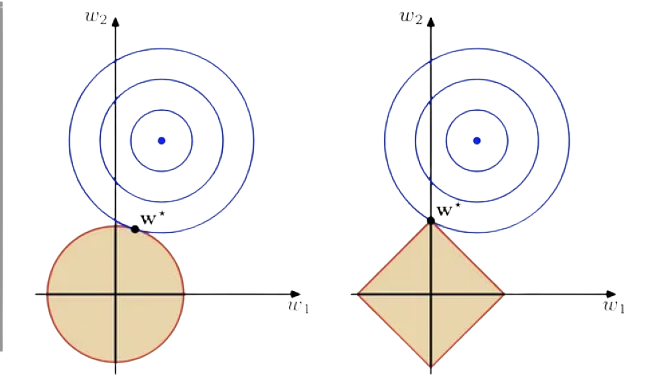
\includegraphics[scale = 0.5]{reg.png}
\end{transitionframe}


\begin{frame}{Регуляризация: общий паттерн} 
	\begin{wideitemize}
		\item  На обучающей выборке мы вносим какую-то случайность 
		\item  На тестовой выборке мы усредняем эту случайность
		\item  Есть много подходов и приёмов, в этой секции мы рассмотрим несколько примеров
	\end{wideitemize}
\end{frame}


\begin{frame}{Dropout}
\begin{wideitemize}	
		\item \alert{Обучение:}  случайно зануляем выходы нейронов
		\item \alert{Тест:} усредняем выход на вероятность 
	\end{wideitemize}
	\begin{center}
		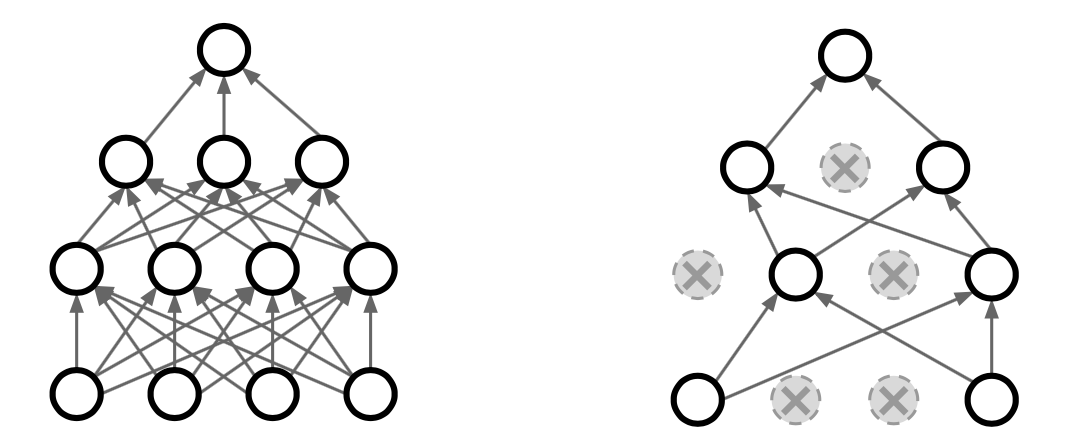
\includegraphics[width=0.55\paperwidth]{dropout_st.png}
	\end{center}
	\vfill %
	\footnotesize
	{\color{blue} \url{http://www.cs.toronto.edu/~rsalakhu/papers/srivastava14a.pdf}}
\end{frame}


\begin{frame}{DropConnect}
	\begin{wideitemize}	
		\item \alert{Обучение:}  случайно удаляем связи между нейронами (зануляем соответствующий вес)
		\item \alert{Тест:} используем все связи 
		\item На практике используется редко 
	\end{wideitemize}
	\begin{center}
		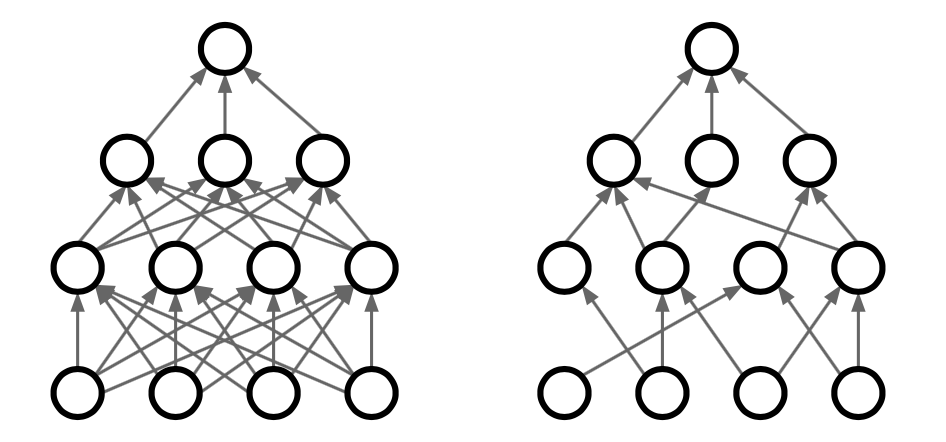
\includegraphics[width=0.5\paperwidth]{dropconnect.png}
	\end{center}
	\vfill %
	\footnotesize
	{\color{blue} \url{http://yann.lecun.com/exdb/publis/pdf/wan-icml-13.pdf}}
\end{frame}


\begin{frame}{Аугментация (Data augmentation)}
	\begin{columns}[T] %
		\begin{column}{.5\textwidth}
		\begin{wideitemize}
			\item Увеличение, уменьшение
			\item Повороты, искажения, приближения
			\item Новые цвета, затемнения
			\item Смена стиля
			\item Нужно ли добавлять сдвиги?  \only<2>{\alert{(нет, вместо них лучше пулинг)} }
		\end{wideitemize}
		\end{column}%
		\hfill%
		\begin{column}{.5\textwidth}
			\begin{center}
				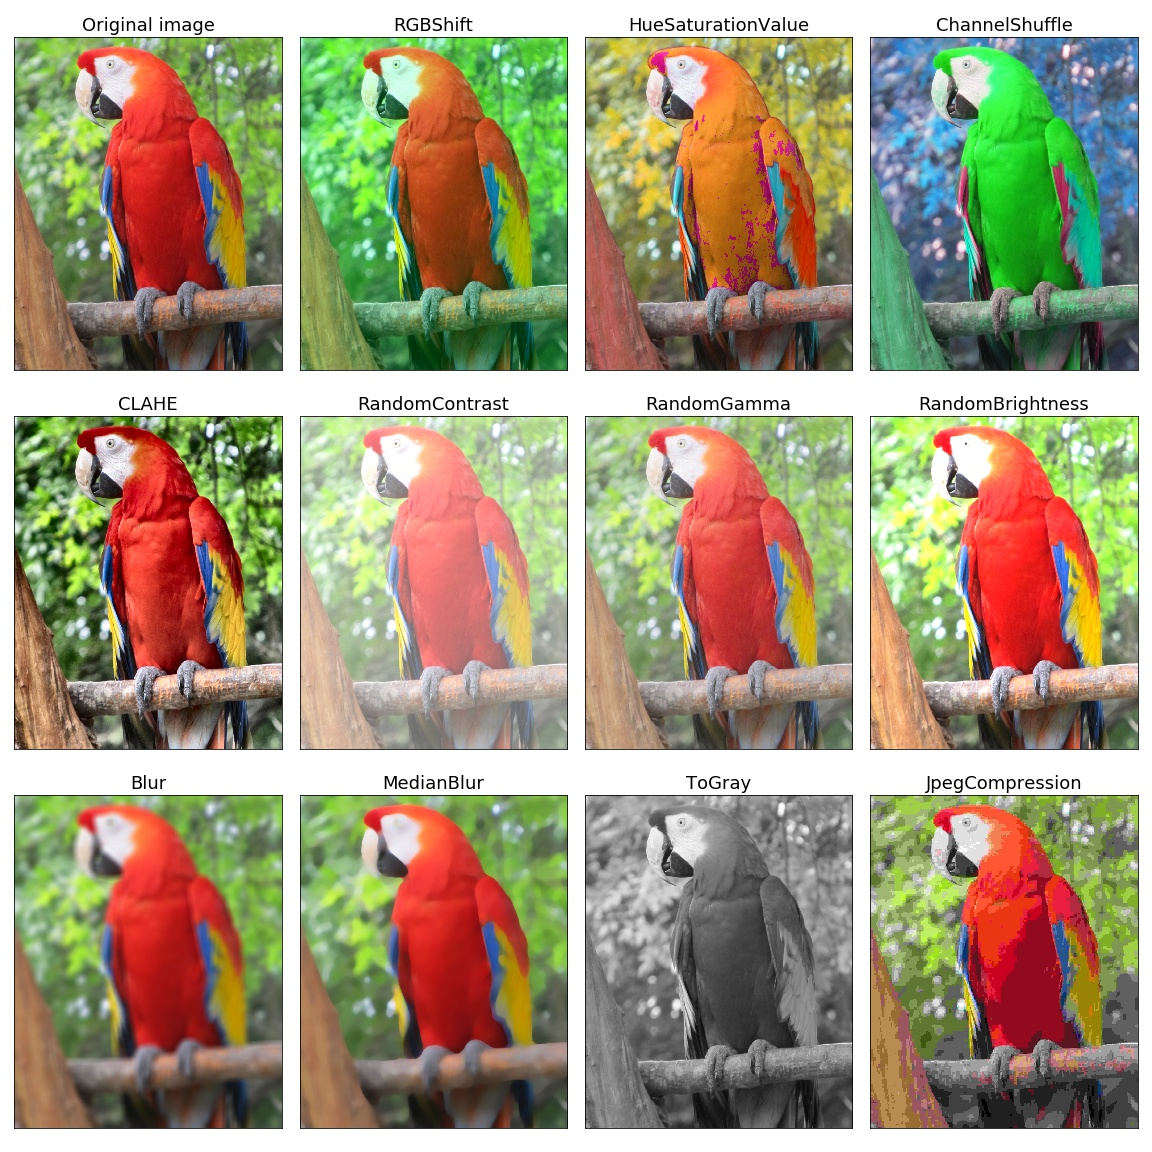
\includegraphics[width=.85\linewidth]{parrot.jpeg}
			\end{center}
		\end{column}%
	\end{columns}
	\vfill
	\footnotesize
	{\color{blue} \url{https://www.tensorflow.org/tutorials/images/data_augmentation}}
\end{frame}


\begin{frame}{Аугментация (Data augmentation)}
	\begin{wideitemize}
		\item Много разных вариантов
		\item «Бесплатное» расширение обучающей выборки
		\item \alert{Обучение:}  случайно применяем к картинкам из текущего батча
		\item \alert{Тест:} делаем несколько аугментаций картинки, применяем сеть к каждой и усредняем предсказания
		\item Для тестовых данных набор аугментаций всегда фиксирован 
	\end{wideitemize}
\end{frame}


\begin{frame}{Вырезание (Cutout/Random crop)}
	\begin{columns}[T] %
		\begin{column}{.5\textwidth}
			\begin{wideitemize}
				\item \alert{Обучение:}  Зануляем рандомные куски картинки 
				\item \alert{Тест:}  используем всю картинку
				\item  Неплохо работает для маленьких датасетов как CIFAR
				\item  На больших датасетах не очень полезно
			\end{wideitemize}
		\end{column}%
		\hfill%
		\begin{column}{.5\textwidth}
			\begin{center}
				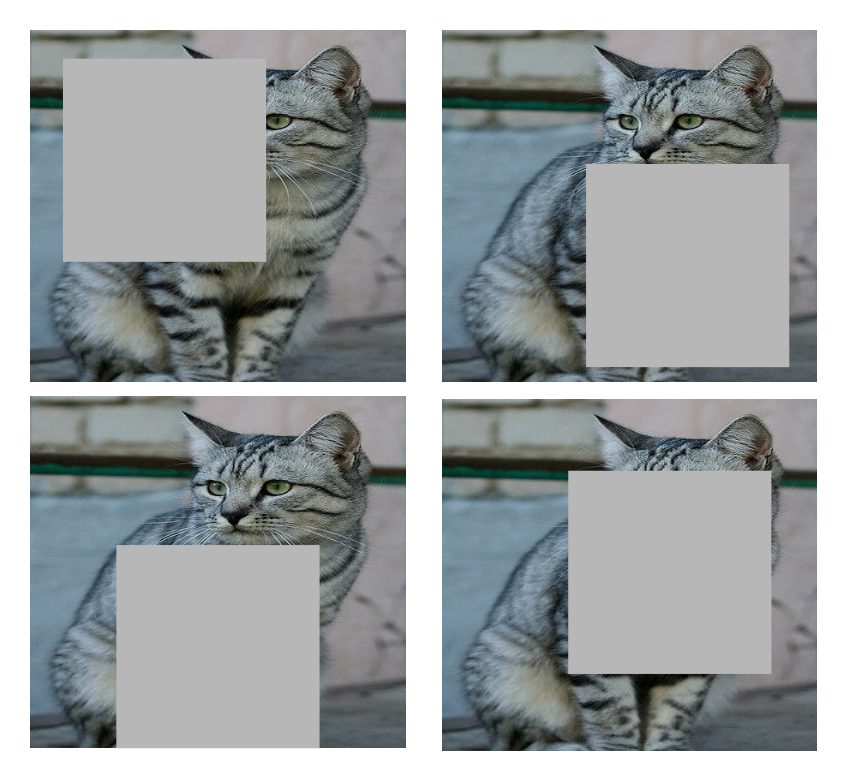
\includegraphics[width=.8\linewidth]{cutout.png}
			\end{center}
		\end{column}%
	\end{columns}
	\vfill
	\footnotesize
	{\color{blue} \url{https://arxiv.org/abs/1708.04552}}
\end{frame}


\end{document}